\chapter{Overview of the IETF Distributed Denial-of-Service Open Treat Signaling (DOTS)}
\markboth{Overview of the IETF Distributed Denial-of-Service Open Treat Signaling (DOTS)}{}
\chaptauthors{Luc Boillat, Fabio Maddaloni, Timo Surbeck \& Jan von der Assen}

%%-----------------------------------------------------------------
\Kurzfassung{%
This is the abstract.
It fits pretty much on one page and is definitely not longer.}

\newpage

%%-----------------------------------------------------------------
\minitoc %table of contents

\newpage

%%-----------------------------------------------------------------
\section{Introduction}

In this chapter, an introduction into Denial-of-Service (DoS) attacks as well as Distributed Denial-of-Service attacks (DDoS) attacks, is given. Thus, first the motivation behind this topic is provided, then some DoS and DDoS techniques are presented. The chapter is finalized with the topic of multivector attacks.

%jan:%
\subsection{Motivation}

There are people who want to harm other people and over time, the possible ways of doing so changed a lot. With the age of digitization and the incoming digital revolution, all different forms of computers became attractive for hackers and other people with bad intentions. Thus, the more computers, smartphones, smart devices or any other device communicating with the Internet are available, the more potential targets arise. With respect to the increasing number of network available devices used every day, it is important to analyze at possibilities against various kinds of attacks.

In 2018, DoS and DDoS attacks combined were the most common type of cyber attacks followed by Man-in-the-Middle attacks, phishing, drive-by-attacks and password attacks \cite{Hostingtribunal-DDoSStatistics, DetectionTechniques}. Despite that, firms, and especially firms only having an online marketplace, faced massive losses and reputation damages when experiencing much downtime. A report from NETSCOUT \cite{Techradar-DDoSStatistics}, a provider for application and network performance management tools, estimates that DDoS attacks could be costing the UK economy more than \£1 billion in 2019 \cite{Techradar-DDoSStatistics}. Furthermore, this report states, that every organization facing DDoS attacks had seen costs of about \£ 140'000 only due to downtime \cite{Techradar-DDoSStatistics}. Lee Mathews, a senior cybersecurity contributor for Forbes Magazine, wrote at that time that the costs of a DDoS Attack can easily climb into several hundreds of thousands of dollars \cite{Forbes-DDoSCosts}.  Despite the fact that it is not clear how these numbers were calculated, it is still impressive and frightening but clearly shows the need for mitigation tools.

The motivation of attackers does change from attack to attack and, probably, there is not one always valid answer, also since the attackers are mostly unknown, but the Reporting and Analysis Center for Information Assurance MELANI of the Swiss government lists extortion, political activism and damaging competitors as the most likely motivations behind such attacks \cite{DDoS-MELANI}. Another paper lists the incentives of attackers as: Financial/commercial gain, revenge, ideological beliefs, intellectual challenge or cyberwarfare \cite{DDoS-MitigationSurvey}. 


\subsection{Statistics \& Famous Attacks}

According to Cisco's annual internet report white paper around 7.9 million DDoS-attacks where observed in 2018 \cite{Cisco-DDoSStatistics}. Believing their numbers, in 2020 the world already faces about 10.8 million attacks annually \cite{Cisco-DDoSStatistics}. Cisco lists an increasing total number of attacks by around 14\% per year, what then brings the result, that in 2023 the total number of attacks will reach about 15.4 million \cite{Cisco-DDoSStatistics}. Thus, the total number of attacks nearly doubles in six years \cite{Cisco-DDoSStatistics}. Other journals and firms draw a less pessimistic image as in 2019 only 8.4 million attacks where recorded compared to the 9.5 millions Cisco lists \cite{ZDNet-DDoSStatistics}. However, even with this number, about 16 DDoS-attacks were launched every minute in 2019 \cite{ZDNet-DDoSStatistics}. 

One of the largest DDoS-attacks ever recorded took place on February 28, 2018 when GitHub, the world famous code management and file hosting platform, was attacked \cite{Metacompliance-DDoSStatistics}. The peak traffic they received was about 1.3 terabits per second (Tbps) \cite{Metacompliance-DDoSStatistics}. The attacker used the memcached vulnerability for this DDoS-attack \cite{Metacompliance-DDoSStatistics}. Shortly after the attack, an unnamed customer of a US-based service provider was attacked with about 1.7 Tbps \cite{Hostingtribunal-DDoSStatistics, Arstechnica-DDoSStatistics}. Compared to this, average mobile internet download speed with Swiss cellular networks was around 27.6 Mbps (or 0.0000276 Tbps) \cite{Statista-MobileInternetSpeed}. The DE-CIX, one of the biggest internet nodes on planet earth in regards of data throughput -- for comparison -- handled a 9.1 Tbps peak in March 2020 \cite{Computerbase-Datarate}.

According to the Kaspersky Lab, UDP flooding was the most used single attack vector in 2018 \cite{Securelist-DDoSStatistics}. HTTP attacks were the second most often used type in 2018 \cite{Securelist-DDoSStatistics}. However, the by far biggest part of attacks were so-called multivector attacks which were used in about 72\% of all attacks \cite{Securelist-DDoSStatistics}. 

Despite the massive load the two previously described firms faced, the average DDoS attack size was about 26.4 Gbps \cite{Hostingtribunal-DDoSStatistics}. Other sources list 12 Gbps, which is less than half of the other amount written about in the last sentence \cite{Helpnetsecurity-DDoSStatistics}. Unfortunately this makes a clear assumption about how big DDoS attacks were in average nearly impossible. Furthermore, not only the amount of data, but also the time span a attack occurs needs to be taken into consideration. Here the longest attack in 2018 lasted about 329 hours which is nearly about 2 weeks \cite{Hostingtribunal-DDoSStatistics, Securelist-DDoSStatistics}. Based on numbers from the Kaspersky Lab only 15\% of all DDoS attacks last longer than 4 hours and only about 3.7\% of all DDoS attacks last longer than 20 hours \cite{Securelist-DDoSStatistics}. Kaspersky list the average duration of DDoS attacks in 2018 to 218 minutes, which is about 3 h 40 minutes \cite{Hostingtribunal-DDoSStatistics, Securelist-DDoSStatistics}. However, when taking the number of 16 launched attacks per minute into account again, this results in about 225 attacks launched every hour. Thus, in every hour, about 34 attacks lasting longer than 4 hours, and around 8 attacks lasting longer than 20 hours were started. When analyzing at these absolute numbers, they definitely show the need of mitigation against such attacks. 

As mentioned in the \textit{Motivation} chapter, the costs for firms and organizations are tremendous. Furthermore, there are reputation damages which are not easily calculated and represented in absolute numbers. Techradar lists the costs for a firm at averaging \£2'140 per minute, Forbes wrote, that the costs can easily go up to several hundreds of thousands of dollars in total at that time \cite{Techradar-DDoSStatistics, Forbes-DDoSCosts}. Thus, providing an absolute value of how much a DDoS attack costs the victim is not possible in this context. The costs for starting an attack, on the other side, can be observed precisely, since, in 2017, DDoS attacks could be bought in the dark web \cite{Securelist-DDoSCosts}. The costs to attack a big online shop for five minutes were about \$5 \cite{Securelist-DDoSCosts}. Another frightening fact is that these stores in the dark web offer DDoS attacks in subscription like manners also called "stresser" or "booter" services \cite{Securelist-DDoSCosts}. Luckily, the FBI and other law enforcing organizations teamed up in 2018 to fight against these services and took down about 15 such DDoS-for-hire platforms \cite{Forbes-DDoSCosts}. The Federal Bureau of Investigation estimates that these 15 providers were responsible for around 200'000 attacks, which shows that there were many people actually using it \cite{Forbes-DDoSCosts}. 

\subsection{DoS Attacks}
One type of cyber attack aimed at any computer is a so called Denial-of-service (DoS) attack \cite{DoS-Explained}. The goal of these attacks is to cripple a computer's resources, or more often a server, such that the intended users cannot use this device and its usual functions anymore \cite{DoS-Explained}. One idea behind a DoS-attack is to flood a device with nearly endless requests \cite{DoS-Explained}. Another one is to use vulnerabilities such that the normal traffic cannot be processed anymore \cite{DoS-Explained}. This will then result in a DoS because the target machine cannot handle the requests anymore, since its capacity is oversaturated \cite{DoS-Explained}. DoS Attacks can occur on Layer 3 \& 4 and also on higher layers like layer 7 which is the application layer \cite{DoS-PCWelt}. Also, they are originated from one single point of action. 

According to Steve Weissman, DoS attacks most often take one of the two following approaches: Flooding attacks or crash attacks \cite{DoS-Norton}.
\begin{itemize}
    \item Flooding attacks are the more common one and occur, when the target gets crippled by an overwhelming amount of traffic \cite{DoS-Norton}.
    \item Crash attacks are less common but as a result of these attacks, the targeted system crashes \cite{DoS-Norton}. With the second approach, attackers transmit bugs exploiting flaws in the targeted system \cite{DoS-Norton}. 
\end{itemize}

Both attack types have in common, that they prevent legitimate users from accessing a server and thus, accessing a website, some applications or data because the servers are overloaded and thus, all capacity is already used  \cite{DoS-Norton, DoS-Comparitech}. Depending on the role of the target machine, this can have tremendous impact. For example, if an online shop is down for a certain time they will obviously not sell anything during this time and not make profit, but if a website providing information during a crisis will be down, people cannot be informed anymore, which is really severe. Since originating and coordinating flooding DoS-attacks is quite simple, they became one of the omnipresent cybersecurity threats \cite{DoS-Comparitech}. Furthermore, the attacks are often very effective and can take some servers down for days or even weeks if there is no appropriate countermeasure applied \cite{DoS-Comparitech}. 

\subsection{DDoS Attacks}
In this subchapter some Distributed Denial-of-Service (DDoS) attacks are described. Furthermore, some numbers about DDoS-attacks are shown.

In the previous chapter, a short introduction into the topic of DoS attacks was given. There is an advanced type of DoS attack occurring in the world, which is called DDoS-attack. This chapter covers differences between a "normal" DoS attack and a distributed one. Furthermore, some metrics and key numbers are presented. 

A DDoS attack is one of the most common attacks nowadays \cite{DoS-Comparitech}. The main difference between a DoS and a DDoS attack is the distributed network from which the attack is started and sent to the target computer. According to Dr. Jose Nazario, a senior security researcher, the two major goals of a DDoS attack are consuming as much bandwidth as possible and overflowing the target server \cite{nazario2008ddos}. Thus, the incentives of DoS and DDoS attacks are similar. 

Since these attacks may come from multiple different sources, filtering and preventing the attack not originated from one single point makes detection and defence against such an attack quite hard \cite{nazario2008ddos}. Based on the Reporting and Analysis Center for Information Assurance of the Swiss government, the data volume of one attack can reach several hundred gigabits, which makes it impossible for many organizations and firms to cope with such attacks without external assistance \cite{DDoS-MELANI}.

Two major techniques used in DDoS attacks are reflection and amplification \cite{ReflectionVSAmplification}. The majority of DoS attacks can be assigned either to one or to both types combined \cite{ReflectionVSAmplification}. Reflection attacks use the same protocol in both directions and the attacker spoofs the IP address of the sending device \cite{ReflectionVSAmplification}. An intermediary server then answers to these requests sending the response not to the attacker's but to the victim's address \cite{ReflectionVSAmplification}. The amplification attack scheme generates a high volume of packets flooding the target's devices, network or websites \cite{ReflectionVSAmplification}. When attacking a target, often reflection with the help of spoofed IP addresses is already used in the amplification process \cite{ReflectionVSAmplification}. With amplification as well as reflection attacks it is possible to achieve a DoS at a target. 

\subsection{Types of DoS \& DDoS Attacks}
In this section important attack vectors (\emph{i.e.}, attack types and techniques) are briefly described and explained. 

Some attack vectors make use of a botnet. A botnet is basically a bunch of computers or other network devices which are malware infected such that they can be controlled from a command server and then act as a network \cite{Botnet-ReadWrite}. Botnets can be used for several different purposes, not only bad ones, but one of the bad intentions is to create and organize a DDoS attack. Unfortunately, a botnet with devices infected by malicious software is not always needed for a DDoS attack because it is also possible to use misconfigured network devices and IP-spoofing without inserting malicious software in the first place \cite{Shadowserver, Cloudflare-SSDP}.

\subsubsection*{ICMP Floods}
ICMP floods, also called ping floods, try to cripple the target server with an overwhelming amount of ping requests \cite{DoS-PCWelt, DoS-Comparitech}. This attack makes use of unconfigured or misconfigured network devices \cite{DoS-PaloAlto, DoS-Comparitech}. These devices are then used to ping every other computer in the network with spoofed packets \cite{DoS-Comparitech}. 

\subsubsection*{SYN Floods}
SYN floods use a vulnerability of the TCP connection, which is often referred to as the three-way-handshake on layer 4 \cite{DoS-Norton, DoS-PCWelt}. In this attack scenario, the attacker floods a server with SYN-packets which then will never be completed, since the attacker will not await the SYN-ACK-response but sends again many SYN-packets instead \cite{DoS-Norton, DoS-PCWelt}. Because they will never be completed, the ports for these connections will be occupied and cannot be used for further requests, which results in the situation where all ports will be occupied and the server will shut down at one point \cite{DoS-Norton}. A legitimate user will not receive a response from the server anymore since the server is down \cite{DoS-PCWelt}. 

\subsubsection*{UDP Flood}
UDP attacks are a way of attacking a target in which many User Datagram Protocol (UDP) packets are sent to a targeted server \cite{Cloudflare-UDP}. For this attack vector, a botnet is needed to start malicious requests with spoofed sender IP addresses \cite{Cloudflare-UDP}. The victim then tries to respond to every packet until it is overwhelmed and drowned in the flood of UDP packets \cite{Cloudflare-UDP}. 

\subsubsection*{Ping-of-Death}
Ping-of-Death attacks are another type of DoS attack which send packets larger then the maximum allowed size, thus larger than 65'535 bytes \cite{PingOfDeath-Cloudflare}. This then causes a buffer overflow and the target machine freezes or shuts down \cite{PingOfDeath-Cloudflare}. This can be effective since some TCP/IP systems were neither designed nor programmed to handle packets larger then the maximal allowed size \cite{PingOfDeath-Cloudflare}. However, this attack type is not very common anymore, since there is a fix for the vulnerability  \cite{PingOfDeath-Cloudflare}. 

\subsubsection*{Teardrop Attack}
With the teardrop attack, another DoS-attack scheme, IP data packet fragments are sent to the network which then tries to recompile these fragments into the original packets \cite{DoS-Comparitech, DoS-Teardrop}. The receiver then cannot reassemble the packets due to a bug in the TCP/IP fragmentation reassembly \cite{DoS-Teardrop}. Then, the fragments overlap another packet causing network devices to crash \cite{DoS-Teardrop}. 

\subsubsection*{SSDP Attack}
For DDoS-attacks, often a botnet is used \cite{nazario2008ddos, DDoS-MELANI}. According to the ShadowServer foundation, a foundation which reveals misconfigured and openly accessible devices with SSDP (Simple Service Discovery Protocol), every device running SSDP in a way that it is externally accessible can be used in DDoS attacks \cite{Shadowserver}. These SSDP-attacks are a reflection-based DDoS attack sending an amplified amount of traffic to the target by using the Universal Plug and Play networking protocol \cite{Cloudflare-SSDP}. This amount of traffic then is overwhelming the target's infrastructure and thus, possibly taking the service down \cite{Cloudflare-SSDP}. SSDP DDoS attacks can be initiated in basically 6 steps \cite{Cloudflare-SSDP}:
\begin{enumerate}
    \item The attacker conducts a scan searching for UPnP (Universal Plug and Play) devices. These devices are needed for a bigger amplification factor. 
    \item All responding devices are put into a list, such that they can be used further. 
    \item A UDP packet with a spoofed IP address is created. The spoofed IP address is the address of the target device.
    \item The spoofed packets are sent to all devices of the list created in step 2. These packets request as much data as possible by setting certain flags.
    \item The devices of the list do not recognize the spoofed IP address belonging to the target device and thus, send data to it. The amount of data sent by one device to the victim can be up to 30 times larger than the attackers request. 
    \item The victim then receives a huge amount of data, basically with an amplification factor of about 30 times the number of devices in the list described at step 2. This possibly results in a denial-of-service causing the legitimate traffic to stop. 
\end{enumerate}

\subsubsection*{NTP Attack}
A so called Network Time Protocol amplification DDoS attack, or short NTP-attack, is a reflection-based volumetric DDoS Attack, which is explained based on CLoudflare's explanation found in \cite{Cloudflare-NTP}. This attack type uses the Network Time Protocol server functionality and its goal is also to overwhelm a targeted device or network. The NTP is used for internal clock synchronization between internet connected devices. Furthermore, it also uses UDP traffic. Thus, the DNS amplification attack makes use of many devices with smaller bandwidth connections, potentially a botnet, to make numerous requests to unsecured DNS servers. With this way, the attacker makes many small requests for large DNS records and then sends these responses to the victim's IP address to overwhelm it. The NTP-attack can be split into four major parts according to Cloudflare \cite{Cloudflare-NTP}:
\begin{enumerate}
    \item UDP packets with spoofed IP addresses are sent to NTP servers, which have their \textit{monlist} commands enabled. The spoofed IP addresses point to the IP address of the target device. The monlist command is a command, which enables administrators to count traffic \cite{Imperva-NTP}. This command answers with a list of, for example, at least 600 hosts that are connected to the queried server \cite{Imperva-NTP}.  
    \item Each of these UDP packets use the \textit{monlist} command in a request. This results in a large response. 
    \item The server responds to the spoofed IP address with the requested data. 
    \item The denial-of-service can happen, when the target server or network then receives this overwhelming amount of traffic and data. 
\end{enumerate}

\subsubsection*{Memcached Attack}
With a memcached DDoS-attack, the goal is to overload the victim with internet traffic \cite{CloudFlare-Memcached}. The attacker spoofs some requests to a vulnerable memcached server \cite{CloudFlare-Memcached}. These servers are designed for speeding up websites and networks during normal visits with a database catching system and use the UDP protocol \cite{CloudFlare-Memcached}. Since the response is typically larger than the request, an effective DDoS attack can be launched when spoofing the requester's IP-address \cite{CloudFlare-Memcached}. A memcached attack basically consists of 4 major steps and does not need a botnet \cite{CloudFlare-Memcached}: 
\begin{enumerate}
    \item An attacker implants a large payload of data into a server, which exposes the memcached service to the internet.
    \item Then the attacker spoofs an HTTP GET request to the server with the IP address of its target. Thus basically the attacker sends a GET request to the server from a faked IP address. 
    \item The server with the exposed memcached service receives the request and thinks that the victim requested the data. Thus it sends the entire response to the target.
    \item The targeted victim is not able to process the huge amount of data incoming from the memcached server, which then results in an overload and a denial-of-service for legitimate service. 
\end{enumerate}

One of the biggest problems of a memcached attack is the magnification factor \cite{CloudFlare-Memcached}. Cloudflare, a firm providing security services as well as distributed DNS-services, mention, that this magnification factor can reach up to 51'000 times the actual data \cite{CloudFlare-Memcached}. This means, that for a 15 bytes request, answers of about 750'000 bytes (750 kB) can be sent \cite{CloudFlare-Memcached}. This tremendous magnification factor and the previous described factor of vulnerable servers makes the memcached attack one of the most used and prime use cases for DDoS attacks against a target \cite{CloudFlare-Memcached}. 

\subsubsection*{DNS Flood}
DNS Floods are another DDoS attack scheme \cite{Cloudflare-DNSFlood}. In this approach, malicious devices in a botnet flood a particular domain's DNS servers in attempt to disrupt DNS resolution for this domain \cite{Cloudflare-DNSFlood}. DNS servers translate easy to remember names to harder to remember numerical addresses \cite{Cloudflare-DNSFlood}. Thus, when this DNS resolution is not working anymore, legitimate traffic cannot find the technical address and thus a denial-of-service occurs \cite{Cloudflare-DNSFlood}. 

\subsubsection*{DNS Amplification}
The DNS amplification attack technique is the second approach using and attacking DNS resolvers \cite{Cloudflare-DNSFlood, Cloudflare-DNSAmplification}. This approach is a reflection-based volumetric DDoS attack and uses open DNS resolvers to overwhelm a target server's possibility to react to legitimate traffic \cite{Cloudflare-DNSAmplification}. As all other amplification approaches, also this one uses the disparity in bandwidth consumption between target and attacker and thus can get huge responses compared to quite small request queries \cite{Cloudflare-DNSAmplification}. This amplification can be fortified when using a botnet with malicious bots requesting the same data \cite{Cloudflare-DNSAmplification}.
Also, this approach uses spoofed IP addresses such that the response get to the target victim which then could go out of business with a denial-of-service \cite{Cloudflare-DNSAmplification}. The process of attack can be divided in four major chunks \cite{Cloudflare-DNSAmplification}:
\begin{enumerate}
    \item UDP packets with spoofed IP addresses are sent to a DNS resolver. 
    \item Each of these sent UDP packets try to achieve the largest possible response such that as much data as possible is sent to the spoofed IP address.
    \item The DNS resolver does its job and sends the requested large amount of data to the spoofed IP address. 
    \item The victim and its network possibly get overwhelmed by the amount of data sent to them which results in a denial of service. 
\end{enumerate}

\subsubsection*{Application Layer Attack}
As described previously, DDoS-attacks can also occur on higher layers than layer 3 or 4 \cite{Cloudflare-ApplicationLayer}. So-called Application-Layer-DDoS-attacks happen, as the name indicate, on layer 7 of the OSI-model \cite{Cloudflare-ApplicationLayer}. These attacks, compared to ones on lower layers, are effective since they also consume server resources instead of only network resources \cite{Cloudflare-ApplicationLayer}. One point of attacking the network as well as the server resources is, that less total bandwidth is needed to achieve the same effect or even a more severe one \cite{Cloudflare-ApplicationLayer}. This is because every time a request is created, the server may have to look up data in the data base or similar things \cite{Cloudflare-ApplicationLayer}. 

\subsubsection*{HTTP Flood}
One of these Layer 7 attacks is a HTTP Flood attack which is also a volumetric DDoS attack \cite{Cloudflare-HTTP}. The overall goal of a HTTP-attack is to overwhelm the target with a huge amount of HTTP requests such that a DoS is the result \cite{Cloudflare-HTTP}. Maximal efficiency can be achieved when using a botnet with malware infected network devices \cite{Cloudflare-HTTP}. This attack scheme can be divided into two different versions \cite{Cloudflare-HTTP}. In the HTTP-GET-attack, the devices in the botnet are requesting data from the targeting server what can lead to an inundation and thus a DoS \cite{Cloudflare-HTTP}. The second approach is done with HTTP POST requests where the bots form the botnet are sending data to the server which needs to handle them correctly \cite{Cloudflare-HTTP}. If the server cannot handle all incoming data appropriately, a DoS can occur \cite{Cloudflare-HTTP}. 

\subsection{Multivector attacks}
The majority of all DDoS attacks use so called multivector attacks. These combined attacks are used, depending on the source, between 72\% and 85\% of all attacks \cite{Hostingtribunal-DDoSStatistics, Securelist-DDoSStatistics, Helpnetsecurity-DDoSStatistics}. Thus, looking at multivector attacks definitely makes sense. 

Multivector attacks are, as the name already indicates, a combination of the previously described attack types \cite{Corero-MultivectorDDoS}. These combinations are used more often by attackers because they are harder to defend \cite{Corero-MultivectorDDoS}. Based on various sources, attackers use often three to four vectors combined \cite{Corero-MultivectorDDoS, Helpnetsecurity-DDoSStatistics}. However, other sources say, that security providers most often fight against DDoS attacks with up to eight vectors used \cite{Corero-MultivectorDDoS}. 

A common combination is to use a mix of amplification vectors as well as traditional ones \cite{Symantec-MultivectorDDoS}. For example, creating a UDP flood in combination with NTP requests as amplification ends in a tremendous amount of data sent to the spoofed IP address \cite{Symantec-MultivectorDDoS}. 

Defending multivector attacks is more complex since they bring some additional challenges which need to be considered into defense mechanisms and thus, they may have a higher success possibility from the attacker's viewpoint \cite{Corero-MultivectorDDoS, Symantec-MultivectorDDoS}: 
\begin{enumerate}
    \item Every vector used in an attack needs to be recognized and fought. This needs to be done as quick as possible and without impacting legitimate traffic.
    \item The defense needs to be applied on different layers at the same time. 
    \item Multivector attacks are mostly additive in terms of bandwidth. This means that the bandwidth used for every vector is added to the whole attack amount which enlarges the amount of traffic faced tremendously. 
    \item Attackers often mix resource exhausting SYN floods from spoofed IP addresses with other vectors. This makes the mitigation and tracking by far more challenging.
    \item Vectors get activated variably. This averts a generalized mitigation. Thus, the best mitigation technique changes also dynamically during an attack. Furthermore, one attack type gets enabled and disabled during an attack period. 
\end{enumerate}

Multivector attacks can be successfully defended with automatic and immediate detection and blockage of all kinds of DDoS attacks \cite{Corero-MultivectorDDoS}. 


\subsection{Mitigation Mechanisms}

As written in previous chapters, DDoS attacks are designed to take down websites, servers and services, by massive amounts of either data or invalid requests. Luckily, the targets are not completely powerless since there are techniques and ideas how to withstand such attacks with none to minor impact for regular, legitimate users. The keyword for this process is called DDoS Mitigation \cite{Cloudflare-DDoSMitigation}. Mitigation refers to the protection process for a target, independent of whether it is a server or a network \cite{Cloudflare-DDoSMitigation}. Simply said, DDoS Protection is what keeps servers and websites online during an attack and hopefully still allows legitimate traffic to access the services such that the damage for the target gets minimized \cite{Cloudflare-DDoSMitigation}. There are multiple various solutions which work different but all towards the same goal: Protection of the target \cite{Wired-DDoSMitigation}.

The process of mitigation depends on the techniques used behind. However, Marc Gaffan, a writer for Wired magazine, lists 4 must-haves and important points to take into consideration for a successful protection of a network or server \cite{Wired-DDoSMitigation}: 
\begin{enumerate}
    \item While the attacker's goal is to damage by not letting legitimate users access the requested services, the users do not care if a service is currently under attack or not. Thus, if they cannot access some services and websites they may never come back if a service is not accessible. Therefore, the first important point is to let legitimate users access a service or website normally despite the fact of an ongoing attack. Legitimate users should never notice the attack, neither by delays, outdated cached content, holding areas or splash screens. Often it is the case, that as soon as attackers recognize that legitimate traffic is still possible, they stop the attack.
    \item If a service is down for legitimate users, the service provider should give them the opportunity of a fail-safe way to complain. 
    It is also important that these messages by legitimate users are addressed as fast as possible.
    \item As listed before, the rise of multivector attacks generated a new problem since a simple mitigation is sometimes not enough to prevent damage. Thus, it is important that all layers are protected and also all attacking bots -- if used for an attack -- are recognized. However, there are also good bots which should have access all time.
    \item Expect the biggest attack possible. Of course, if a service provider is only running a small business with a tiny online shop with only a few users, it is not to be expected that a record breaking attack is hitting this service. However, since the amplification techniques are used widely, mitigation should still work for unexpected high attack volumes. 
    \item Basically, there are two major stages of a mitigation: Detecting and defending an attack. Another paper writes about three major steps: detection, defence and IP traceback \cite{DetectionTechniques}. If there are no tools capable of detecting that some services are under attack, it is nearly impossible to defend the target in an appropriate way. Detection is somewhat tricky since the it should work instantly if a service is going to be attacked but otherwise stay in the background and not slow down or influence legitimate traffic in another way. If there is no detection, the best protection defensive mechanisms are useless since they will not become triggered. 
\end{enumerate}
All these points need to be taken in consideration if a mitigation tool is used, because only focusing on some of them will probably not bring the desired outcome \cite{Wired-DDoSMitigation}.

Detection, mitigation and response can be done at different places on the attack routes between the attacker and the target \cite{DDoS-MitigationSurvey}. A DDoS attack can be thought of a funnel, where attacks are originating at multiple sources and narrow down to the target, which makes it easier to detect DDoS attacks the "nearer" they are related to the target \cite{DDoS-MitigationSurvey}. This is in contrast to the desire of responding to an attack as "far" away as possible, meaning as "near" as possible to the actual source, which results in a trade-off situation \cite{DDoS-MitigationSurvey}. There is a tendency that the nearer a defense mechanism is applied, the more legitimate packets are dropped \cite{DDoS-MitigationSurvey}. 

In their paper, Saman Taghavi Zagar et al. classify defense positions network- \& transport-level attacks into source-based, network-based, destination-based and hybrid, while application layer attacks are classified into destination-based and hybrid, since layer 7 attack traffic cannot be accessed in layer 2 or 3 devices on its way \cite{DDoS-MitigationSurvey}. Furthermore, attack prevention (before), attack detection (during) and attack source identification (after) is used as chronologic classification \cite{DDoS-MitigationSurvey}. This reveals that a comprehensive DDoS mitigation needs to consider all these spatial and chronologic categories since there is not a one-fits-all solution \cite{DDoS-MitigationSurvey}. Here the techniques and intentions behind services for these classifications are shortly explained: 

\subsubsection*{Source-based} 

These mitigation services are applied as near to the attack's source as possible \cite{DDoS-MitigationSurvey}. Thus, most often, they can be placed at a source's edge router of the local network or at the access router of an autonomous system which is connected to the source's edge router \cite{DDoS-MitigationSurvey}. They are not entirely effective because (a) the attack's source(s) can be distributed, (b) the differentiation between legitimate packets and malicious is difficult and (c) the motivation to install such services is low since it is unclear who pays the services \cite{DDoS-MitigationSurvey}. The following source-based mitigation approaches are all based on the paper by Saman Taghavi Zagar et al. \cite{DDoS-MitigationSurvey}:
    \begin{itemize}
        \item Ingress/Egress filtering at the sources' edge routers: Filtering of ingress and egress traffic based on source addresses at a attacker's edge router. There are problems with the detection of spoofed IP addresses and there is a huge overhead resulting in a narrow application range. 
        \item D-WARD: This aims to detect DDoS attack flows by comparing the measured network traffic with predefined normal traffic flow. Thus, attacks are recognized, if they mismatch the predefined scheme. For example: if there are no TCP-ACK recognized, something could be wrong.
        \item MULTOPS (Multi-level Tree for Online Packet Statistics) and TOPS (Tabulated Online Packet Statistics) are heuristics and data-structures which can be used to detect and filter DDoS flooding attacks. It is done with the proportionality of Ingres and Egress traffic which results in the fact, that significantly disproportional traffic in one direction indicates the source or target of an attack. However, MULTOPS is a lucrative target for memory exhaustion attacks since it is very memory consuming. TOPS are used for improving the accuracy and reducing the false alarm rate. Furthermore, incoming and outgoing traffic is not always proportional (e.g. because of streaming or downloading data). This is also used by attackers to create a more proportional ratio. 
        \item Reverse Firewalls try to protect the outside internet form a malicious packet coming from the inside network. They actually work in the opposite direction than a normal firewall. This is, for example, done by limiting the forwarding rate for packets or analyzing the senders IP-address. Unfortunately, a reverse firewall is quite stable and cannot be changed dynamically.
    \end{itemize}
    
\subsubsection*{Destination-based}
Detection and response is mostly done at the attack's destination \cite{DDoS-MitigationSurvey}. It is similar to the source-based approach either done on the edge router or at the autonomous system of the target \cite{DDoS-MitigationSurvey}. Unfortunately, most of the destination-based mechanisms cannot accurately detect and mitigate the attack before it is already using resources \cite{DDoS-MitigationSurvey}. The following approaches for destination-based mitigation are all based on the paper by Saman Taghavi Zagar et al. \cite{DDoS-MitigationSurvey}:
    \begin{itemize}
        \item IP Traceback mechanisms are tracing back the IP addresses to their true source IP, rather than the ppoofed one. Therefore, packet marking and/or link testing is used. Both possibilities have various deployment and operational challenges. It is needed, that enough routers support traceback since otherwise it is not effective. Also, traceback messages can be faked which some attackers exploit.
        \item The Management Information Base (MIB) data is a collection of various packet and routing statistics which help victims to recognize DDoS attacks when continuously analyzed. This can also be used to adjust the network parameters. 
        \item Packet Marking and Filtering mechanisms are used to mark legitimate on every router passed such that the victim's edge router can let them pass. These filters can become ineffective, if an attack is to heavy. Currently used ones are History-based IP filtering, Hop-count filtering and Path identifier.
        \item Packet dropping based on the level of congestion is used to drop suspicious packets when the network is overloaded up to a certain level. A common approach is called Packetscore. 
    \end{itemize}
    
In contrary to source- \& network-based mitigation techniques, destination based mechanisms can also be used against Application layer DDoS attacks \cite{DDoS-MitigationSurvey}. Since most application layer protocols are organized as client-server models, these mitigation approaches are mainly used to protect the servers directly at their electrical positions with anomaly detection, various drops and/or limits \cite{DDoS-MitigationSurvey}. The Application layer mechanisms listed in Saman Taghavi Zagar et al. contain following approaches \cite{DDoS-MitigationSurvey}:
\begin{itemize}
    \item Defense mechanisms against Reflection/Amplification attacks are mostly deployed at the server-side with the goal of detecting malicious traffic. Therefore, DNS amplification detection mechanisms and algorithms to detect authorized users are applied. 
    \item DDoS-Shield mechanisms use statistical methods to apply rate-limiting as the primary defense against HTTP floods. This mechanism consists of a suspicious assignment mechanism (for continuous value assignment) and a DDoS-resilient scheduler (which works as a rate-limiter and uses the continuous value to reschedule a session's request). 
    \item Anomaly detector based on hidden semi-Markov model is used to describe the dynamic of the access matrix to detect an attack. The drawback of this is its tremendous complexity. 
    \item Defense Against Tilt DDoS attacks (DAT) monitors the users instant traffic volume, session behaviours and other things during a connection session to determine malicious users. 
\end{itemize}
    
\subsubsection*{Network-based}
The goal of this approach is to stop an attack in the network between source and target and help the source- and destination-based mechanisms to do their work properly \cite{DDoS-MitigationSurvey}. These approaches usually lead to high storage capacities and a processing overhead at the routers \cite{DDoS-MitigationSurvey}. This gets even worse, if the mitigation process becomes redundant \cite{DDoS-MitigationSurvey}. Reducing redundancy enhances the communication effort \cite{DDoS-MitigationSurvey}. The following approaches for network-based mitigation are all based on the paper by Saman Taghavi Zagar et al. \cite{DDoS-MitigationSurvey}:
    \begin{itemize}
        \item Router-based packet filtering assumes that an unexpected source address may indicate a spoofed IP address and the packet can be filtered. However, carefully selected IP addresses or genuine IP addresses are not filtered. 
        \item Detecting and filtering malicious routers with the help of special anomaly detection protocols was proposed to detect malicious routers. Here, explicit communication between routers is needed and spoofed packets cannot be filtered. Since the communication can be faked, the attacker can use packets to misidentify the target as malicious router which is even worse from a victim's perspective.  
    \end{itemize}
    
\subsubsection*{Hybrid (Distributed) mechanisms} 
The previous three described approaches (source-, destination- \& network-based) can work without much coordination and cooperation amongst the various involved parties and detection as well as mitigation is done mostly by each of the parties \cite{DDoS-MitigationSurvey}. On the contrary, hybrid mechanisms are deployed at multiple locations and there is usually coordination and cooperation between the locations \cite{DDoS-MitigationSurvey}. The following approaches for hybrid and distributed mitigation are all based on the paper by Saman Taghavi Zagar et al. \cite{DDoS-MitigationSurvey}:
\begin{itemize}
    \item Hybrid packet marking and throttling/filtering mechanisms usually place the attack detection mechanisms near the target and the packet filtering is located near the attack sources. Furthermore, sometimes the victim uses a forward-throttling some routers away from it to slow down the forwarding rate. These mechanisms only influence the malicious packets and let the legitimate ones pass as intended. Used mechanisms are: Aggregate-based Congestion Control and Push-back, Attack Diagnosis and Parallel Attack diagnosis or TRACK.
    \item Defensive Cooperative Overlay Meshes are distributed frameworks enabling service and information exchange among all defending nodes. All nodes should collaborate and coordinate such that the mitigation is successful and effective. The nodes in this approach are specialized for their particular purpose (e.g. detection or trace-back), depending on the virtual distance to the source. Thus, it is important, that they can communicate all the time, despite the force of the attack. 
    \item CROSSACK is a mechanism built on all of the border routers of the edge networks and based on some assumptions (border routers need to have ingress/egress filtering mechanisms and must be able to prevent IP spoofing). The software used, therefore, is assumed to be able to stop DDoS attacks.
    \item Capability-based mechanisms let the victim explicitly authorize and allow the traffic it wants to receive. The routers along a path check whether the traffic is legitimate. If not, \emph{i.e.}, there is no permission that a system can send data to the victim, the data flow is stopped. These mechanisms are always active and their processing and memory overhead are high. 
    \item Active Internet Traffic Filtering as a filter-based mechanism bring the possibilities to deny all traffic by default and only allow the traffic which belongs to established network-layer connections. There is also the opposite possibility which allows all traffic by default and explicitly denies undesirable traffic. 
    \item StopIt is a mechanism which allows receivers to install network filtering services blocking undesirable traffic. It uses Passport as authentication for sources which prevents IP address spoofing. Since StopIt uses own servers, they may also become the target by floods, making the system attackable. 
\end{itemize}

Also, hybrid techniques can be used against application layer attacks \cite{DDoS-MitigationSurvey}. They are listed here based on Saman Taghavi Zagar et al. \cite{DDoS-MitigationSurvey}:
\begin{itemize}
    \item Speak-up is a technique, which asks all its clients to increase the volume of traffic sent, because then attackers, too, need to increase it, which uses more bandwidth also at the attacker's side. If an attacker already uses most of its bandwidth, it cannot send more data and thus gets revealed. The legitimate users, not using all bandwidth, can drastically increase the data volume. The goal is that the legitimate users crowd out the malicious ones. This technique is only usable against session flooding attacks and not in case of request flooding or an asymmetric attack. 
    \item Defense and Offense Wall (DOW) is a mechanism using the Speak-Up technique combined with an anomaly detection method based on K-means clustering. This should be able to detect session flooding, request flooding and asymmetric attacks. Similar to Speak-Up, the legitimate users increase their rate such that they become more likely to be served, resulting in dropping suspicious and rising legitimate sessions. 
    \item Differentiate DDoS flooding bots from humans can also help to distinguish between legitimate and malicious users. For example, Completely Automated Public Turing Test to tell Computers and Humans Apart, better known as CAPTCHA) are employed, which currently cannot be solved by computers. The disadvantage is here, that the users need to solve puzzles, which increases delay and difficulty for legitimate users. Additionally, web crawlers cannot access sites using CAPTHAs either, such that search engines are hindered from indexing web pages. 
    \item Admission control and congestion control regulate the number of concurrent users accessing online services. This works by port hiding and resource allocation on legitimate users. This approach uses a challenge server, which could also become a target for DDoS attacks by itself. 
    \item Trust Management Helmet (THM) uses trust to differentiate between legitimate users and attackers. The idea is that the connection to legitimate users should be prioritized and thus kept online before trying to identify all attack requests. This works with cryptographically secured licenses for legitimate users. 
    \item Hybrid detection based on trust and information theory based on metrics is another approach which filters suspicious flows based on the trust value score by the client. This score is maintained by the server, based on previous visits. After this, an entropy is applied for final filtering of suspicious flows. 
\end{itemize}

\subsubsection*{Before the attack}
As mentioned previously, mitigation approaches can be categorized spatially and chronologically. DDoS attacks can be fought best by prevention, \emph{i.e.}, DDoS mitigation already takes place before the attack is actually started \cite{DDoS-MitigationSurvey}. Most of the prevention approaches try to fix security vulnerabilities and can be deployed at the attack's source, in intermediate networks, at the target or at a combination of them \cite{DDoS-MitigationSurvey}. However, prevention alone does never completely remove the threat of DDoS attacks, mainly because there will always be new attack vectors \cite{DDoS-MitigationSurvey}. The following attack prevention mitigation techniques are all based on Saman Taghavi Zagar et al. \cite{DDoS-MitigationSurvey}:
\begin{itemize}
    \item System \& Protocol security mechanisms are put into place to increase the overall security of a system. This can be done by preventing access to machines for illegitimate users, fixing bugs, updating protocols, installing patches or removing unused software. Thus, an up-to-date system is very important. 
    \item Fail-safe protection makes use of possibilities when something goes wrong by e.g. redundant infrastructures and services, business and disaster management, etc.
    \item Resource allocation \& accounting: Provide enough resources to counter a DDoS attack and control the access for users based on privileges and behaviours. 
    \item Reconfiguration mechanisms change the topology of the victim's network or the intermediate network by adding more resources and/or isolating the attacker's network.
    \item Installing firewalls and improving intrusion detection and prevention systems: End hosts should install and use intrusion detection and prevention systems. 
    \item Local filters, such as ingress/egress filters, IP filtering, hop-counting or packet filtering, can be used to block attack flows before the bombardment is running. 
    \item Load balancing and flow control can be used for improving performance and mitigation. Furthermore they can be used to prevent servers from going down. 
    \item Server-side specific security considerations: Policies or security mechanisms can help against server vulnerabilities especially for layer 7 attacks. 
    \item Service providers can also have strategies which bring a better identification of legitimate users. For example by applying dynamic pricing of resources \textbf{[missing end of sentence]} % TODO: Add end of current sentence
\end{itemize}

\subsubsection*{During the attack}
Attack detection is done during the attack and can also be applied in the same places like the prevention mechanism described in the previous chapter. Some detection methods detect DDoS attacks based on the load-level of the network links, others based on anomalous traffic patters in layers 3,4 \& 7 \cite{DDoS-MitigationSurvey}. Some mechanisms use data mining and/or artificial intelligence for more accurate detection \cite{DDoS-MitigationSurvey}. Therefore theses mechanisms learn about normal traffic and detect anomalous traffic, if they are trained well enough \cite{DDoS-MitigationSurvey}. Defending against an attack should be done at the earliest point possible and as near as possible to the attacker's location \cite{DDoS-MitigationSurvey}. Defending at the source or in the intermediate network has advantages since the detection mechanisms are less vulnerable for DDoS attacks targeting them and the detection is more concealed \cite{DDoS-MitigationSurvey}. But there are big challenges, namely: The lack of DDoS detection mechanisms and the lack of collaboration \& cooperation among all distributed defense mechanisms \cite{DDoS-MitigationSurvey}. The latter would mainly be used for increasing accuracy, increasing performance efficiency and decreasing redundant (and often unnecessary) tasks \cite{DDoS-MitigationSurvey}. 

As already mentioned before, application layer DDoS attacks can only be detected at the destination because of protocol designs \cite{DDoS-MitigationSurvey}. But it is possible to fight against attacks with in-depth architecture analysis of extractable layer 2 \& 3 features \cite{DDoS-MitigationSurvey}. 

After an attack has been detected, it needs to be defended successfully \cite{DDoS-MitigationSurvey}. For a successful mitigation the source of the attack should be identified and the attack traffic blocked \cite{DDoS-MitigationSurvey}. This leads to the focus of minimizing the attack impact while maximizing the availability of the service for legitimate users \cite{DDoS-MitigationSurvey}. Furthermore, it is important that providers and others cooperate with each other since otherwise a successful mitigation is nearly impossible \cite{DDoS-MitigationSurvey}. 

The identification of the real attack's source is very important and often done with IP traceback mechanisms  \cite{DDoS-MitigationSurvey}. The second important point is applying an appropriate response which is often done with throttling or packet filtering on upstream routers \cite{DDoS-MitigationSurvey}. 

\subsubsection*{After the attack}

After the attack is over, it is important to evaluate the impact, the defense and prevention for next time \cite{DDoS-Radware}. Here it is important that the attack is evaluated in detail and not just superficially \cite{DDoS-Radware}. This includes also understanding and estimation of the costs of the DDoS attack, which then helps to estimate how much should be spent on defense next time \cite{DDoS-Radware}. For a better protection, weak spots need to be identified and improved \cite{DDoS-Radware}. During this step, false positives should also be taken into consideration, since one goal is to provide continuous service for legitimate users despite the fact that this service is under attack \cite{DDoS-Radware}. 


\subsection{Mitigation services and solutions}
The previous subsection has introduced a number of mitigation techniques that can be used to mitigate a DDoS attack and a classification thereof. Such a mitigation technique can be part of a larger solution that provides support for the lifecycle of a DDoS defense. In the following paragraphs we will therefore introduce a number of solutions that embody some type of DDoS mitigation which can be used to protect from attacks. We will consider both solutions from the industry as from academia and highlight current trends relevant to the development of an open signaling protocol. We will do so by employing a categorization that distinguishes between mitigation scenarios that are either centralized, distributed or decentralized. Additionally, we will outline whether the approach is executed on the vicitm's premise or off-premise.

\subsubsection{On-Premise Mitigation}
Whenever the victim mitigates the attack at the destination site where the attack is targeted at we can see many of the destination-based mitigation techniques as described previously. These scenarios are by nature centralized and on-premise since all operations from mitigation through mitigation are executed in the customers domain. The mitigation techniques such as for example using a firewall to filter unwanted traffic can be used to deter small attacks. It is likely that such measures are not applicable for complex or large-scale attack.
If the victim employs multiple sites for the mitigation process we can classify such a scenario as distributed since multiple systems have to be orchestrated carefully. A number of more complex approaches that were explained previously such as "Speak-up" and "Bots vs Humans" would fall into this category and could have potential to deal with larger attack than with the centralized scenario.
Both of these scenarios however could benefit from a standardized protocol which is used for the orchestration of complex attacks.

\subsubsection{Off-Premise Mitigation}
Commercial DDoS Mitigation Services (DMS) come in two variants, distributed or decentralized, with the distributed ones having a very large number of customers. Jonker et al. have proposed a methodology which allows one to look at DNS records to determine how many services point to a mitigation service. This redirection can be seen as a presence of ongoing mitigation provided by a DDoS mitigation provider. Their findings concluded that the rise in announced records pointing to a mitigation service exceeded the global rise in number of announced records, from which they concluded a positive increase in adoption of such services.
Jonker et al. investigated the adoption of nine large DDoS mitigation services such as Akamai and CloudFlare which can be considered to apply distributed mitigation. Our literature review revealed little information about how the signaling to such services works and if there are negative consequences to their design. However, the findings in the following paragraphs are important to consider when discussing the approach taken in DOTS.

As mentioned in the methodology to measure adoption rate, the ability to do traffic redirection using DNS is an important feature. This type of traffic redirection is often used if one wants to protect a single web service. The customer of such a protection service could be an operator, domain registrar or web hoster.

Alternatively, traffic can also be redirected by means of doing BGP prefix announcements. This way, all the traffic directed towards the customer is routed to the mitigation service. There, the traffic is filtered and the sane traffic is routed to the customer using some sort of tunneling mechanism. This type of protection strategy is most often used when one wants to protect a whole network. These two diversion techniques seem to target different stakeholders, nevertheless many stakeholders support both approaches.

DDoS Protection services may be used in a continuously protecting manner or on demand. For both of the protection manners both traffic diversion strategies can be seen in practice. How a mitigation request is signaled to the DDoS provider is not detailed but it at least provides evidence for the demand of doing on-demand attack protection.

To summarize, providers of distributed DMS continue to gain attraction, have proprietary or manual interfaces and finally they require some form of traffic diversion. Thus, a standardized protocol for signaling would provide a number of advantages if used as an interface. However, as we can see from the current adoption of these services it would need to be compatible with current traffic diversion techniques. Given the increasing adoption rate of these DMS we can assume that there should be at least some interest in the problem DOTS tries to solve \cite{dps-adoption}.

The former services had embodied a similar architecture where there was some entity detecting the attack and another one filtering the attack traffic, hence the classification as distributed system. However, with the scale of current attacks that can reach multi-terabit traffic levels, the infrastructure of such a scrubbing service could be overwhelmed as well. Cisco further argues that such attacks requires orchestration of multiple network operators in a decentralized manner. Their proprietary solution aimed at peering network providers is said to be already deployed in a number of locations \cite{ciscodecentralizedddos}.

The general idea of cooperative DDoS defense is to have a decentralized view on the attack and to mitigate at the outgoing link of one or more parties. The advantage of this approach is that multiple domains have the possibility to analyze the attack traffic, which opens solutions such as the source-based mitigation systems introduced in the previous chapter.

Another implementation which can be considered to be open was developed by Rodrigues et al., where a blockchain was used to handle financial aspects of an attack mitigation. The exchange of attack information is not handled on the actual blockchain \cite{blockchain-collaborative-defense}. Thus, it leaves out specific details on how a reliable signal channel under attack conditions can be achieved.

These decentralized approaches may open a number of advantages in mitigating DDoS attacks. Firstly, they could increase the capacities and secondly they might provide a different perspective which may allow for more efficient detection of such attacks. Given their complex and decentralized nature such services could make use of a standardized protocol which may increase the compatibility between a large number of providers. However, such a protocol would need to be able to reflect the relationships and operations as they would be required with a decentralized approach.

%%-----------------------------------------------------------------
%\section{Background}
%Some text about this chapter's content. This chapter will be more technical than the previous \emph{Introduction} one. 
%
%jan:%

%For example:
%\begin{itemize}
%    \item Autonomous systems -> rfc1930
%    \item How traffic is routed between ASes ->  rfc4271
%    \item How protection from unwanted traffic normally works and why it does not work with DDoS attacks 
%    \item SDN?
%    \item Anycast routing
%    \item Related standards / protocols such as CoAP -> rfc7252
%      -> similar to HTTP, but over UDP, subset of HTTP, URIs, DTLS, RESTlike functionality for constrained devices, maybe outline the most important terminology since this would be visited again in the protocol design (if we choose to detail the design): \url{https://tools.ietf.org/html/rfc7252#section-1.2}
%    \item RESTconf -> rfc8040
%    \item What is the IETF, their goals and incentives.
%    %jan: %
%    For the presentation we can maybe also include a who-is-who in the internet world? E.g. IANA, IEEE, IETF, ITU etc
%    \item Maybe also which organizations are involved in the dev of tihs standard, e.g. NTT
%\end{itemize}{}

\section{IETF DOTS}
The previous chapters provided an introduction to DDoS attacks and existing mitigation approaches. This chapter introduces the efforts of the DOTS working group. Specifically, we give an introduction to the terminology followed by the use cases in which the standard should prove useful, thus, showing the objectives of the working group. The remaining subsections will introduce the architecture and design of the standard which shows how the standard is supposed to solve the problems mentioned before.

\subsection{DOTS}
% What is DOTS and how does it work 

%\textrightarrow maybe introduce the basic components? % TODO TS
%In order to explain the way how DOTS intends to solve the problem of DDoS mitigation we will introduce the most important terminology which will be used in the following chapters about requirements and the DOTS architecture.?

DOTS stands for DDoS Open Threat Signaling and is a standard currently developed at IETF (Internet Engineering Task Force). DOTS can be described as a set of methods and principles to coordinate defensive measures applied by mitigating peers. As such, DOTS is specified to strictly exist as a standard focused on signaling, which means that in currently published standard document drafts state actual mitigation-related as well as other responsibilities as being out-of-scope with respect to DOTS. The following basic DOTS components are all based on the official IETF DOTS Architecture document \cite{dots-architecture}:

\begin{itemize}
    \item \textbf{DOTS client:} The DOTS client can be described as the downstream DOTS party, which is attached to a target (\emph{i.e.}, server hosting a web-service) standing under attack.
    \item \textbf{DOTS server:} DOTS servers are the counterpart of DOTS clients, in such that they are affiliated with a mitigation service and therefor represent the upstream DOTS party.
\end{itemize}

\begin{figure}[H]
\label{fig:DOTSarchitecture}
\fbox{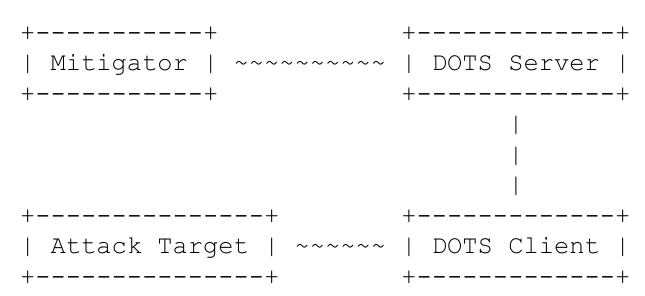
\includegraphics[scale=0.35]{Seminar-Template/Talk7/images/DOTS_Architecture.png}}
\centering
\caption{Main DOTS Parties \cite{dots-architecture}}
\end{figure}

\paragraph{Signal channel} To enable communication among upstream and downstream DOTS parties, a resilient connection -- in DOTS called signal channel -- must be put into place. DOTS clients attached to an Attack Target use this signal channel to request mitigation support, while the same channel is used by DOTS servers to transmit information about ongoing mitigations back to DOTS clients. The DOTS signal channel is precisely specified in a separate document (\cite{dots-signal-channel}), enabling standardization and thus, compatibility among different solutions implementing the DOTS standard.
\paragraph{Data channel} The DOTS data channel is an optional connection between DOTS parties to exchange DOTS configuration and policy information, \emph{e.g.} for DOTS clients to send accept-lists holding addresses of trusted sources to their DOTS server. It is assumed, that data is only transferred over the data channel during "normal" conditions, \emph{i.e.}, not during ongoing attacks. Thus, there is no requirement for the DOTS data channel to be as resilient as the signal channel.

\begin{figure}[H]
\label{fig:DOTSarchitecture}
\fbox{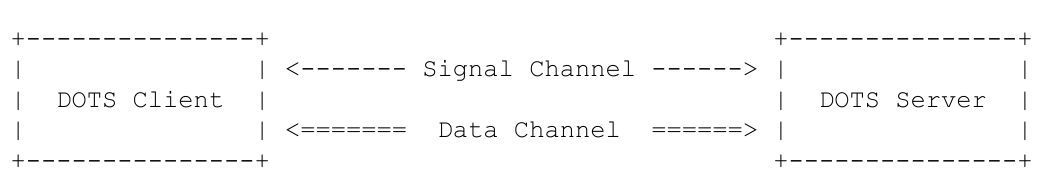
\includegraphics[scale=0.3]{Seminar-Template/Talk7/images/DOTS_Interfaces.png}}
% => Added the use cases as goals section since its thedd only document I found where overall objectives were introduced.
\centering
\caption{DOTS Interfaces \cite{dots-architecture}}
\end{figure}

\subsection{Goals and Use Cases}\label{goals}

The goals of the DDoS Open Threat Signaling working group have been expressed in a number of use cases defined as an Internet-Draft. 

\begin{itemize}
\item The first objective of the standard is to create a solution which is open. This is in contrast to current commercial solutions which are largely proprietary. These commercial solutions are still the basis of most protection services. The drawback of using such services is that these systems are incompatible with each other. Once a user selects and uses a mitigation service, they will usually experience a lock-in effect. Given that these systems do not share common interfaces, large efforts towards the operation and provisioning are introduced.

\item Secondly, the complexity introduced in the previous paragraph can increase if multiple systems have to be coordinated which can be challenging both in technical and non-technical matters. This complexity can lead to the mitigation being costly as well as being inefficient as the complexity of the system can be a hurdle.
\end{itemize}

This is where the DOTS protocols aim at improving the communication channels used in such a mitigation scenario. The proposed protocols should improve the interoperability of existing DDoS mitigation solutions. These protocols should support the whole life cycle of a mitigation process including detection and specification of attacks as well as the request for mitigation \cite{dots-use-cases}.

We will introduce the three major use cases from which concrete requirements towards the respective components in the architecture of DOTS were derived. These requirements are later described in more detail in section \ref{sec:requirements}.

In the first use case the mitigation may be provided through an upstream ISP and the attack target would already be an existing customer of the ISP. The customer may be a residential customer but a professional customer like an enterprise or cloud service would be more likely. This relationship between ISP and customer brings the advantage that the ISP is already on the path towards the client network. With this relationship, two scenarios are possible where DOTS could be applied. Firstly, the ISP could provide mitigation services on request from the customer. Secondly, the ISP has a perspective on the network that allows the identification of the customer as the source of an attack. Thus, it allows to handle two scenarios for the customer which would both be undesirable, namely being victim or source of an attack. However, the document hints towards the first scenario being more likely. Figure \ref{fig:isp-mitigation} outlines how such a scenario could work. Here we can see an enterprise network operating a Web server which will be attacked by a botnet.

The selection of a type of attacker is arbitrary and does not greatly influence the scenario. The important bit is that all the traffic towards the victim is routed through one or more ISPs. Once the victim notices this attack the ISP can be requested to perform a mitigation. This may even happen automatically when a certain traffic pattern is observed, for example a certain throughput. As one can see in the diagram, the ISP has a beneficial position to perform the mitigation since it stands between the botnet and the victim. The ISP would then filter the attack traffic and continuously provide status information until the victim decides to stop the mitigation. 

There are a few things to note with this scenario which characterize the overall solution. First, this scenario requires that both parties need to have the required components installed and need to have agreed to form this relationship. This involves the deployment, configuration of the DOTS server and client. Further, the actual detection and classification of the attack has to be done by the enterprise network, \emph{i.e.}, the victim. This would still involve some manual intervention or the presence of an Intrusion Detection System (IDS) which both still holds a certain complexity.
The next thing to note is that although the mitigation is performed by the ISP the enterprise is still required to control the orchestration and execution of the attack. This is being done by continuously receiving and evaluating status update messages from the ISP. This information is crucial to have for the victim since it needs to eventually signal the termination of the attack mitigation. This means that the attack mitigation is not completely automated or that some system needs to be properly configured to this automatically. This is presumably still complex since the operator or IDS needs to know the infrastructure, such that it can properly signal the requested protection of specific services. Next, it is important to keep in mind that the signal channel needs to be maintained. This can be on the same link where the DDoS attack takes place or through a dedicated connection. For example, a mobile network connection may provide the signal channel. Similarly, if the enterprise network is multi homed, \emph{i.e.}, if the victim has multiple upstream ISPs this adds complexity since the DDoS mitigation has to be orchestrated by the client through its upstream providers.

\begin{figure}
    \centering
    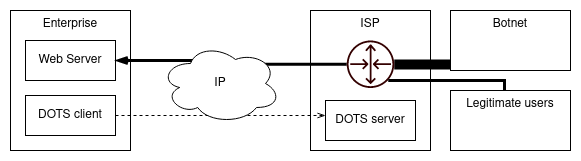
\includegraphics[width=16cm]{Seminar-Template/Talk7/images/ISP-DMS.png}
    \caption{Active Mitigation service provided by an upstream ISP during a DDoS attack}
    \label{fig:isp-mitigation}
\end{figure}{}

If the ISP does not offer mitigation services or if the potential victim wants to use a different third-party mitigation service, a few key differences arise in that scenario compared to the previous one. We will outline how the components and relationships need to be shaped for this use case and which consequences arise from doing so. Under normal circumstances, the traffic to the enterprises service,  a Web Server, will be routed directly through the ISP as expected. Given an attack takes place which needs to be detected and classified by the victim, the victim needs to signal to the mitigation service that it requests help in mitigating the attack. This request will usually be routed through the same link where the attack occurs, however, other links could also be used. Given that the mitigation service and enterprise have previously agreed to handle such requests, the mitigation service will then handle and filter the traffic. The sensible traffic would be forwarded towards the upstream ISP which will then route it to the destination service. 

Many of the elements are similar to the previous use case. The obvious difference is that only the victim and the mitigation provider have to run the components that understand the DOTS protocol and only these two entities need to have a contract for DDoS mitigation. The main difference with respect to consequences for the overall procedure is that the mitigation service might not lie on the routing path between source and target service. This requires that traffic needs to be routed to the mitigation service, or rather that such a routing be advertised. Multiple solutions to do so exist and two are mentioned more prominently. First, one could change the traffic routing on the network layer by making a BGP announcement. Therein, the previously announced route would be withdrawn and the new route that would now include the mitigator would be announced as part of the network layer reachability information. Both of which can be done in a single BGP route resulting in IP traffic being routed to the mitigation service once the routing advertisements have led to a convergence \cite{bgprouting}. Alternatively, the victim could advertise the rerouting on the application-layer using the DNS protocol. Naturally, both approaches provide different perspectives on the infrastructure and have different advantages and disadvantages. For example, with the DNS-based approach, one could redirect individual services running on the same machine behind the same IP address. One caveat shared by both of the approaches is that loops need to be avoided. This is especially important since the routing from mitigator and victim needs to remain intact during the attack. For example, consider the case where all traffic destined towards the victim is automatically routed towards the mitigator. Assuming that the mitigator sends a mitigation update to the enterprise, if this is not handled properly, the ISP in the center might redirect the traffic back to the mitigator as announced previously. Not mentioned in the draft is the absence of attack source detection, where the enterprise might have been compromised and used as a source to create a DDoS attack \cite{dots-use-cases}. With the previous use case this could be covered, but for this use case we assume it would be complex, since traffic is only routed through the mitigator during an active mitigation. Although the exact implementation is left outside of the standard, we have adopted the BGP-based routing to give an overview over the data flow and components in figure \ref{fig:3rdparty-mitigation}.

\begin{figure}
    \centering
    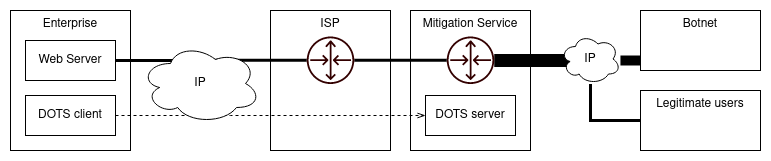
\includegraphics[width=16cm]{Seminar-Template/Talk7/images/3rdparty-DMS.png}
    \caption{Active Mitigation service provided by a 3rd party DDoS mitigation service during a DDoS attack}
    \label{fig:3rdparty-mitigation}
\end{figure}{}

The previous use cases showed two scenarios where there was only one DOTS client requesting a mitigation from one mitigation provider running a DOTS server. The use cases were simple, such that they could even be employed for a residential customer. Within an enterprise network such a mitigation would probably involve more complexity. At first, the actual detection of a DDoS attack would require the orchestration of a number of devices in a non-trivial way. Secondly, it would be imaginable to have a mitigation service running inside of the enterprise's own network. This service would provide the attack mitigation towards a service for a specific attack volume. Ideally, this mitigation service would be able to perform both roles: Acting as a DOTS server for the orchestrating client (1) while also being able to act as a client to request help from yet another mitigation provider (2) once the volume exceeds the supported traffic. A use case depicting both use cases can be seen in figure \ref{fig:ddos-orchestration}, where a recursive structure of DOTS clients and servers, both inside and outside of the enterprises network is shown. Note that compared to the previous figures, the visualization contains a snapshot of an attack where all components for an attack mitigation are in place. However, the currently ongoing DDoS attack is not yet mitigated on any level.

\begin{figure}
    \centering
    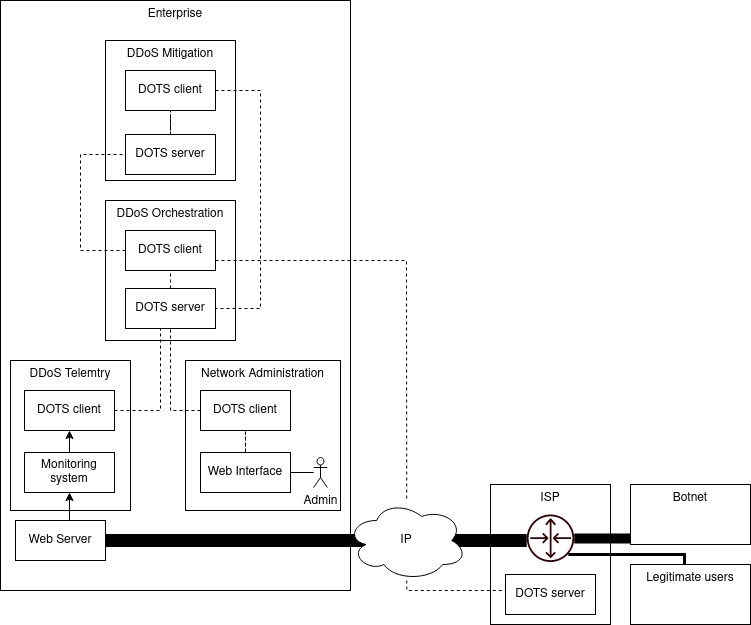
\includegraphics[width=13cm]{Seminar-Template/Talk7/images/ddos-orchestration.png}
    \caption{Infrastructure for a recursive mitigation through a number of local and external DOTS clients and servers.}
    \label{fig:ddos-orchestration}
\end{figure}{}

Since the components resemble a hierarchical structure, we will describe them bottom-up, starting with the infrastructure that is monitored for incoming DDoS attacks. We will describe the components inside of the enterprise network. The external mitigation services are not relevant for this use case, such that one of the two previous approaches could be used. In figure \ref{fig:ddos-orchestration} the ISP directly provides the external mitigation.

On the lowest layer, we have the infrastructure that is being monitored for anomalies in traffic behavior. The standard defines neither interfaces nor protocols but we can assume a number of devices that implement network management protocols. These devices would be observed by the monitoring and telemetry systems which also act as DOTS clients. Thus, it is possible for a set of devices to request mitigation once a specific threshold is reached. We will call this subsystem the DDoS telemetry subsystem, which we consider on the same hierarchical level as the Network Administration subsystem. This one consists of a network administrator interacting with the same DOTS server by means of a web interface which uses a DOTS client to connect to the aforementioned server. Interestingly to note is that with this a manual operation of the use case is still considered reasonable.

Both of these clients would connect to the DDoS orchestration system which provides a client and server. However, this subsystem does not provide an actual mitigation component. Its main purpose is the central management of the previously mentioned clients. For example, it would be thinkable that there is both an automated monitoring component and a manual operator requesting mitigations. Actual mitigations would be handled by a DDoS mitigation subsystem which again needs to be able to respond to mitigation requests. Thus we can imagine the actual mitigation request being handed upwards until this component is reached. For specific attacks it could directly handle the mitigation on its own, for example by reconfiguring some component in the infrastructure layer. For some other attacks it might need help itself and would do so by requesting help from the DOTS server present in the orchestration system. This one could then again forward the mitigation request to a different mitigation provider. This one should provide other capabilites, such as the ones outlined in the previous use cases. Therefore, the heart of the orchestration which would be the orchestration subsystem which handles an attack through a series of interactions with different mitigation providers \cite{dots-use-cases}.

\subsection{Requirements}\label{sec:requirements}
We introduce the most important requirements that led to this architecture. The requirements we are about to introduce have been defined as part of RFC 8612, which is not an Internet Standards Track specification and merely captures the consensus of the IETF community \cite{rfc8612}.
The requirements that presented in this chapter are a subset of the complete set of requirements published under that RFC. Thus, the requirements presented should provide necessary context and background information for the subsequent chapter where the DOTS architecture is introduced. We will also follow the structure of that report which outlines requirements to different parts of the system. First, we introduce general requirements, which are directed towards the standard and its implementation as a whole. Next follow the requirements to the most important component of the system, the signal channel. Following this, the data channel which will have different properties than the signal channel is described in terms of requirements. Finally, we will introduce security and data model requirements. An introduction to congestion control considerations for the elements introduced before will conclude the requirements to the DOTS standard.
\subsubsection{General requirements}
The first requirements presented in the RFC are two quality requirements and two functional requirements. We think they all are essential to understand the stakeholders, their context and consensus which is why we will present all of them.
First, it is expressed that the standard embodied through protocols and data models needs to be extensible. Two reasons are mentioned to stress this necessity, first it should encourage the adoption and incorporation of proprietary DDoS defense systems. This shows us that the DOTS standard tries to focus merely on the communication between mitigators and victims and that only the communication is required to be of open nature but not so the actual mitigation. Secondly backwards compatibility is a desired outcome of an extensible implementation.

The second quality requirement requires the signaling protocol to be resilient and robust. This is not surprising, since DDoS attack aim at disrupting the infrastructure with respect to these two properties. What this implies for the standard is that the protocol must function even when messages are lost and that different techniques should be considered to increase these attributes. For example, the architecture should consider if multiple servers can be operated to increase robustness and resilience. However, this requirement does not dictate a concrete requirement what exactly needs to be done, \emph{i.e.}, the previous example is only a hint on what to investigate.

The functional requirements described towards the standard as a whole mandate that bulk data exchange is possible. Sending larger messages with attack information should enable a better attack response. However this is in conflict with the resilience requirement which dictates smaller message sizes. Thus a requirement for a separate, less resilient channel which may carry more information is defined. The fact that clients may send information to aid in the actual mitigation stems from the requirement that clients should hint about possible mitigation techniques if possible. However, it is not mandated that the mitigators actually make use of this information. This detail is left up to the implementation.

A final functional requirement is specified, namely that there should be a mechanism in place that could handle misconfigurations which would otherwise end up in a loop. Both the detection and resolution of such a loop should be covered \cite{rfc8612}.

\subsection{Signal channel requirements}
This section of the RFC defines concrete requirements for the operation of the signal channel. The signal channel is the channel which must remain operable even under attack conditions since it is used as the main communication channel between attack target and mitigator. The requirements specification defines the highest number of requirements for this part of the architecture from which we conclude that it must be of high importance to the overall system. It is also important to note that all requirements but one in this section are defined as "absolute requirements" as defined in BCP14 \cite{bcp14}. We will thus summarize the requirements to this channel since it appears to be a critical component.

The first requirement specifies that a common transport layer protocol is to be used for this channel. They recommend that UDP should be used for the signal channel and that TCP should be supported for cases where the underlying network policy mandates its use. The use and support of these protocols is not stated as absolute requirement and therefore leaves some room for the implementation.

The next requirement is again specified as absolute necessity and leaves little room for other implementations. This requirement mandates that a message that is to be sent over the signal channel should never get fragmented by the underlying network. This must be achieved by two things. First, it mandates that the speakers within DOTS must send messages that are smaller than the maximum transfer unit \cite{rfc8612}. The maximum transfer unit is the largest packet size that the underlying network can carry without having to fragment it to pass it over some link \cite{rfc791}. It is important to note that this MTU should be adhered to while considering the payload of the DOTS message, byte overhead, transport-level header and security overhead. Thus the DOTS agent needs to be aware of all of those details above the network layer and split the message into smaller messages if necessary.
Finally, it requires that the maximum transfer unit of the underlying unit is learnt through the usual operations. If this is not supported by the underlying network or not feasible to do, the specification defines a default of 576 bytes to be used.

Next, it is specified that channels between clients and servers need to support bidirectional communication. Following, the exchange of heartbeat messages is introduced which makes sure that NAT and firewall traversal is maintained and that absence of such a message can be used to influence the mitigation  operation. From this we can also see that deployment forms involving NAT elements should clearly be supported.

Next follow requirements for the basic operations provided through DOTS. First that mitigation requests can be made and that a mitigation status can be obtained. Although the request of a mitigation is only described with one sentence it appears to be an important operation to be supported. Further it is specified which information about a currently ongoing mitigation should be obtainable, \emph{e.g.} the number of packets blocked. Once a mitigation request is received, the server may handle it with an appropriate mitigation or they may redirect the channel. If the server decides to handle the mitigation request two additional properties of a mitigation request become of importance. Firstly, the lifetime of a mitigation request after which the mitigator should terminate the mitigation if this period was not extended with an updated message from the client. However it should be possible to request indefinite mitigation lifetime from a server which does not have to be granted by the mitigator. The next crucial property of a request is the scope for which they wish attack mitigation. From the mandatory scopes defined we can derive support on the application layer as well on the network layer. On the network layer it is mandatory to support IPv4 and IPv6 prefixes. On the application layer it is mandatory to understand both domain names as well as URIs \cite{rfc8612}.


\subsection{Data channel requirements}
As previously described, the signal channel can be considered the most important communication channel of the DOTS standard. This becomes clear when considering the rather few requirements defined for the data channel. The data channel is not required to provide similar robustness under attack conditions, however, the transport on the data channel should still support message ordering. The main requirement to the data channel is to support resource configuration and additional scope definition \emph{e.g.}, letting clients define drop-lists \cite{rfc8612}, similarly to how it would be done on a Firewall.

\subsection{Security requirements}
The requirements made towards DOTS with respect to security can easily be summarized since these are common security requirements with which the reader may already be familiar with.
Firstly, DOTS is required to allow both parties, the client and server to mutually authenticate against each other with an authentication procedure left to implementations. Additionally, messages directed towards the server must be authorized so that unauthorized clients will be rejected. Once messages are being exchanged, their integrity, confidentiality and authenticity need to be ensured. Given that privacy-sensitive information is likely to be contained, the channels are also required to provide data privacy and integrity as well as protection against replay attacks \cite{rfc8612}.

\subsection{Data model requirements}
The data model requirements were specified to support the operations and qualities described in the previous sections in a way which fosters successful implementations.
Requirements are defined towards how the data model is to be structured, versioned and how it is related to other protocols. Further it specifies which of the properties described before have to be represented. This covers elements such as the mitigation lifetime, status, scope, signal loss and heartbeat \cite{rfc8612}.

%%-----------------------------------------------------------------
\section{Architecture}

%\begin{itemize}
%    \item Description of the architecture.
%    \item Components
%    \item Operations
%    \item .. Sessions, Signaling (recursive)
    %jan:%
%    \item Maybe also different topologies / deployment forms?
%    \item Manual vs automated operation?
%\end{itemize}

This chapter gives an overview of the main architectural concepts of DOTS, based on the official IETF DOTS architecture document (\cite{dots-architecture}). More specifically, initially the most essential abstractions with respect to relationships among DOTS agents is outlined, followed by an introduction to several signaling-related scenarios enabling efficient DOTS agent collaboration.

\subsection{DOTS agent relationships}
The DOTS standard foresees, that DOTS agents (DOTS clients \& servers) communicate with each other via a signal channel as well as optionally, a data channel, which both are mutually authenticated. DOTS does not dictate any specific authentication method \emph{resp.} technique, hence it is an official requirement for DOTS implementing systems to set up the authentication process beforehand, \emph{i.e.} prior to a signal channel being operational and DOTS servers receiving mitigation requests from DOTS clients. Once the authentication process has been successful, both DOTS server and client then establish a DOTS Session in terms of a client-server relationship. However, simple client-server affiliations are not sophisticated enough to implement on top of them distributed, collaborative DDoS mitigation systems. Thus, DOTS introduces a third DOTS agent type, namely DOTS Gateway.

\subsubsection{DOTS Gateway}
DOTS gateways can be described as DOTS client/server hybrids, as they occur as DOTS servers for their downstream agents (\emph{i.e.}, a DOTS client or another DOTS gateway) and as DOTS clients for their upstream agents (\emph{i.e.}, a DOTS server or another DOTS gateway). As such, DOTS gateways are positioned in a DOTS server's domain (\emph{i.e.}, server-side gateway) or -- on the contrary -- in the domain of a DOTS client (\emph{i.e.}, client-side gateway). In either case, DOTS distinguishes between aggregating \emph{resp.}, non-aggregating gateways: The former type terminates several discrete clients' connections and bundles them into a single (\emph{resp.}, differently accumulated) DOTS session towards its upstream agent, while the latter unchangedly passes through its downstream agents' sessions to its upstream agent.

\begin{figure}[H]
\centering
\subfigure[Non-aggregating]{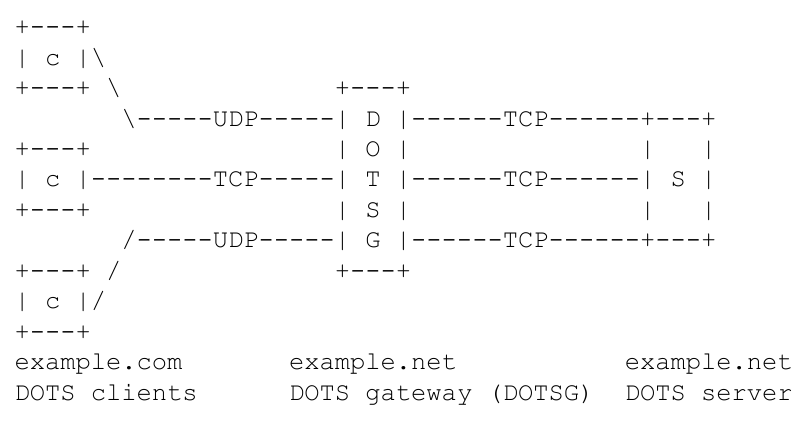
\includegraphics[scale=0.26]{Seminar-Template/Talk7/images/ServerSideWOaggregGateway.png}\label{fig:Ex_Im}}
\hfill
\subfigure[Aggregating]{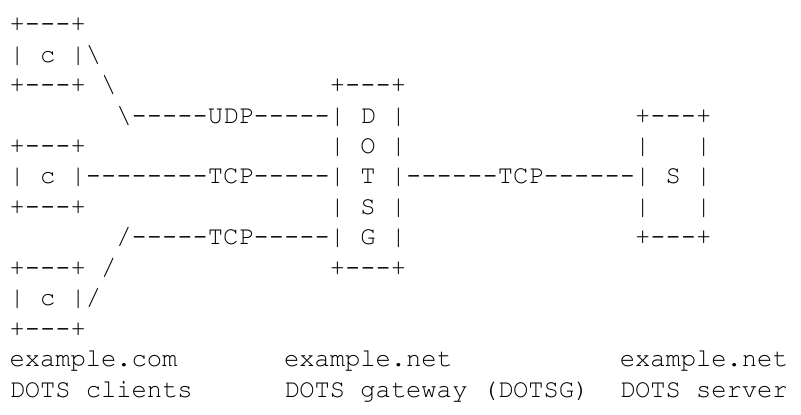
\includegraphics[scale=0.26]{Seminar-Template/Talk7/images/ServerSideWaggregGateway.png}\label{fig:Ex_Im2}} 
\caption{Server-side DOTS gateways (DOTSG) \cite{dots-architecture}}
\end{figure}

\begin{figure}[H]
\centering
\subfigure[Non-aggregating]{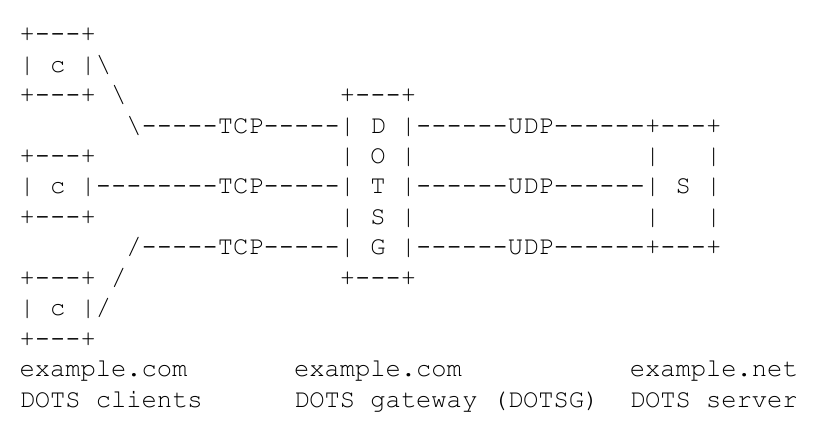
\includegraphics[scale=0.26]{Seminar-Template/Talk7/images/ClientSideWOaggregGateway.png}\label{fig:Ex_Im}}
\hfill
\subfigure[Aggregating]{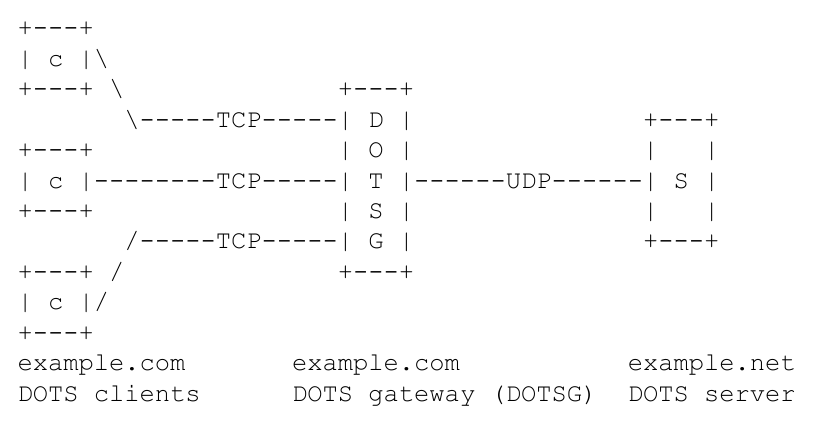
\includegraphics[scale=0.26]{Seminar-Template/Talk7/images/ClientSideWaggregGateway.png}\label{fig:Ex_Im2}} 
\caption{Client-side DOTS gateways (DOTSG) \cite{dots-architecture}}
\end{figure}

\subsubsection{DOTS Sessions}
As mentioned earlier, DOTS sessions are established by setting up a bilaterally authenticated data exchange among DOTS agents. Thereby, DOTS session traffic may flow over the DOTS signal channel, data channel, or both. Signal channel sessions are specified to run over a single TCP \emph{resp.}, UDP session, while using TLS or, the UDP-compatible DTLS as security protocol. Data channel DOTS sessions -- on the other hand -- are specified to use a single TLS-encrypted TCP connection.

In order to maintain DOTS sessions, agents periodically send heartbeat signals to each other. In the case of a DOTS agent observing an extended absence of heartbeat signals from their counterparts, DOTS sessions can be considered as terminated. It is left up to DOTS agent operators on how to configure and set-up the DOTS session maintaining heartbeat exchange mechanism. However, the DOTS architecture document states a clear caveat in advising DOTS agent operators to not configure heartbeat signal intervals too short, which would result in a high heartbeat frequency. The reason therefor is that sending an extensive amount of heartbeat signals could potentially result in unintended denials of service at the receiver, which would obviously defeat the purpose of DDoS mitigation services implementing DOTS.
\subsection{Modes of Signaling}
This section covers more advanced modes of signaling, which -- in contrast to simple direct signaling among a single DOTS client and server -- offer the benefit of letting DOTS agents collaborate, \emph{e.g.} in case of exhaustion, device- or network-failure, etc.

\subsubsection{Redirected Signaling}
Redirected signaling addresses scenario, in which a DOTS server aims at redirecting a DOTS client to a different server. Some examples for such situations include DOTS servers reaching a maximum number of sessions with clients, outage of a mitigator affiliated with a DOTS server (\emph{e.g.} due to exhaustion), or, maintenance to DOTS agents \emph{resp.}, the network path in-between. The illustration below depicts a basic DOTS client redirection:

\begin{figure}[H]
\label{fig:redirectedSignaling}
\fbox{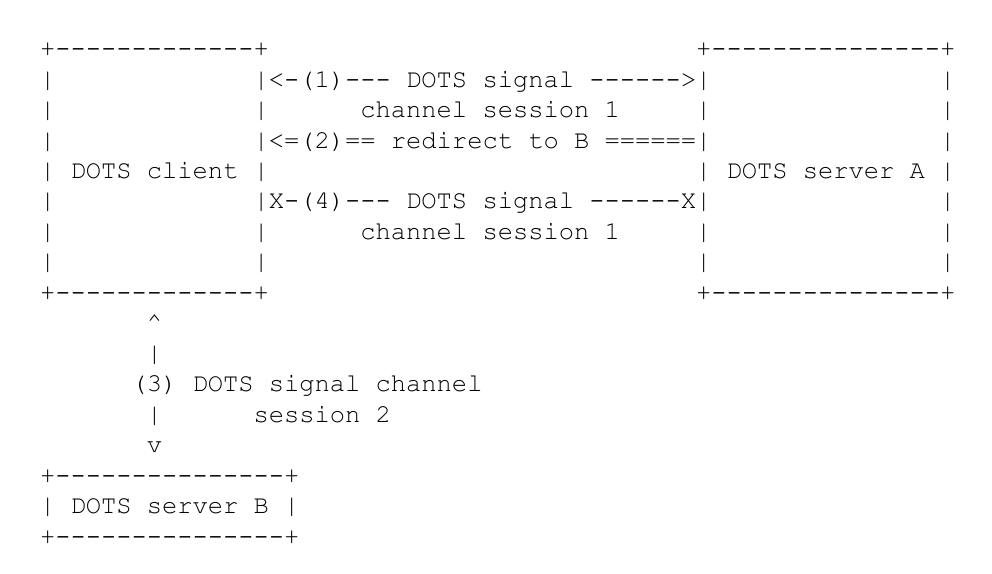
\includegraphics[scale=0.3]{Seminar-Template/Talk7/images/RedirectedSignaling.png}}
\centering
\caption{Redirected Signaling \cite{dots-architecture}}
\end{figure}

(1) incorporates an ongoing DOTS session between a client and server A. At (2), DOTS server A signals to the client it should redirect and establish a new session with server B, to which the client obeys to, as shown at (3). Finally, server A ceases to send heartbeat signals to the client, which is why eventually, the session is terminated, as indicated at (4).

\subsubsection{Recursive Signaling}
Recursive signaling is another mode considering scenarios where DOTS servers cannot meet clients' demands anymore. Here, the aim is however different, in such that the goal is not a redirection of the client (and thus the server quitting its mitigation responsibility), but rather distributing mitigation activities by building DOTS server domain federations. This is especially reasonable when a DOTS server gets overwhelmed by a request to mitigate a very severe attack, such that the resources needed for a successful mitigation would clearly exceed service level agreements (\emph{i.e.}, preliminarily negotiated with a DOTS client): Instead of then dropping the client's request for mitigation, the DOTS server -- being also a DOTS client -- recurses the client's request to a separate DOTS domain, with the expectation of building a federation allowing for cumulative attack mitigation.

The principle of recursive signaling is depicted in the following figure, in which server \texttt{Sn} serving client \texttt{Cc} is actually part of a DOTS gateway (\texttt{Gn}) such that in the advent of mitigation requests exceeding the capacities of domain \texttt{example.net}, \texttt{Cn} can request mitigation support from server \texttt{So} residing in a different administrative domain, \emph{i.e.}, \texttt{example.org}.

\begin{figure}[H]
\label{fig:recursiveSignaling}
\fbox{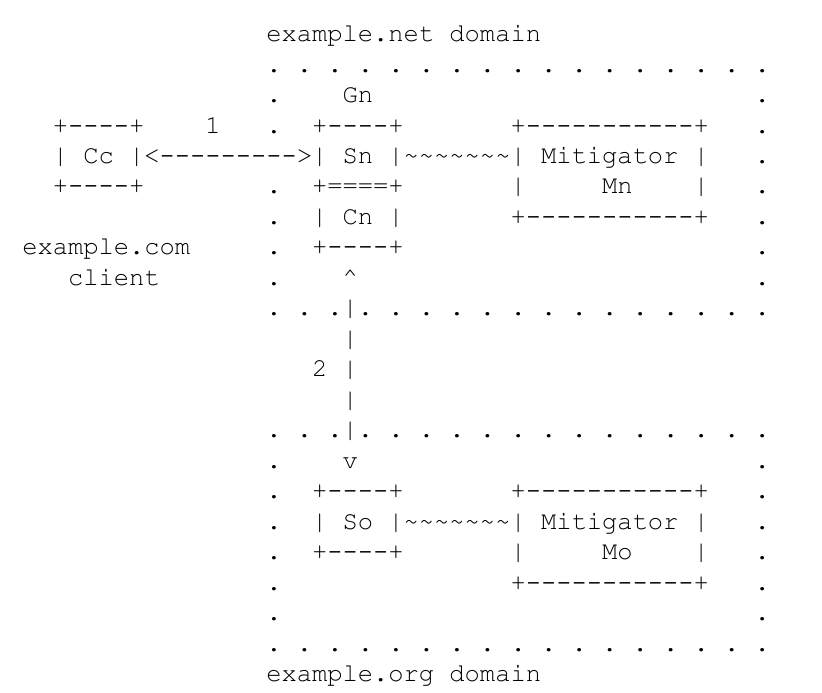
\includegraphics[scale=0.3]{Seminar-Template/Talk7/images/RecursiveSignaling.png}}
\centering
\caption{Recursive Signaling \cite{dots-architecture}}
\end{figure}

\subsubsection{Anycast Signaling}
Although anycast addresses resolving to DOTS servers are not an official requirement, the DOTS standard highlights several benefits of using them: The basic idea behind anycast signaling is equipping DOTS servers with an anycast service address known by every DOTS client. Thereby, DOTS servers themselves become responsible for re-routing clients to the unicast address of an available DOTS server. 

The main benefits of using anycast in DOTS are firstly, the possibility to use simplified DOTS client configurations, since DOTS clients are only required to know the common anycast server address. This clearly simplifies the process of server discovery from a DOTS client perspective. Secondly, regional- \emph{resp.} customer-specific deployments of DOTS are installed more easily, as the responsibility of resolving to unicast DOTS server addresses is moved away from DOTS clients. Finally, arguably the biggest advantage is that when using anycast server addresses, signaling traffic coming from clients is spread across entire DOTS domains, which provides more resiliency and reduces attack surface.

\iffalse
%jan:%
\section{Protocol design}
Maybe we can also show the proposed design for the protocol, e.g. the signal channel? I think this would be a nice next chapter after the architecture and would give some basis to evaluate current implementations.

\begin{itemize}
    \item Protocol stack / Used technologies like CoAP, RESTCONF
    \item Port considerations and server discovery
    \item CoAP URIs
    \item Maybe also go into a bit of more detail for one of the operations and walk through a full example E.g. this is how a mitigation request would look like:
A client would send a CoAP PUT the URI blablabla with the following body, where target-prefix does ... and so on?
\end{itemize} 

\begin{verbatim}
    
     {
       "ietf-dots-signal-channel:mitigation-scope": {
         "scope": [
           {
             "target-prefix": [
                "string"
              ],
             "target-port-range": [
                {
                  "lower-port": number,
                  "upper-port": number
                }
              ],
              "target-protocol": [
                number
              ],
              "target-fqdn": [
                "string"
              ],
              "target-uri": [
                "string"
              ],
              "alias-name": [
                "string"
              ],
             "lifetime": number,
             "trigger-mitigation": true|false
           }
         ]
       }
     }
\end{verbatim}
Or in the presentation we could walk through an actual example if its too abstract otherwise, e.g. first show a diagram of how the actors relate with prefixes etc and then how the request would look like e.g:
This would indicate to the mitigator that the web services of some prefixes are under attack pls do something about it:
\begin{verbatim}
         Header: PUT (Code=0.03)
     Uri-Path: ".well-known"
     Uri-Path: "dots"
     Uri-Path: "mitigate"
     Uri-Path: "cdid=7eeaf349529eb55ed50113"
     Uri-Path: "cuid=dz6pHjaADkaFTbjr0JGBpw"
     Uri-Path: "mid=123"
     Content-Format: "application/dots+cbor"

     {
       "ietf-dots-signal-channel:mitigation-scope": {
         "scope": [
           {
             "target-prefix": [
                "2001:db8:6401::1/128",
                "2001:db8:6401::2/128"
              ],
             "target-port-range": [
               {
                 "lower-port": 80
               },
               {
                 "lower-port": 443
               },
               {
                  "lower-port": 8080
               }
              ],
              "target-protocol": [
                6
              ],
             "lifetime": 3600
           }
         ]
       }
     }
\end{verbatim}
Then later the client could ask the mitigator about a mitigation state using the GET verb and he would see that the mitigator blocked thousands of TCP packets and 0 UDP packets etc etc.

\begin{verbatim}
    
   {
     "ietf-dots-signal-channel:mitigation-scope": {
       "scope": [
         {
           "mid": 12332,
           "mitigation-start": "1507818434",
           "target-prefix": [
                "2001:db8:6401::1/128",
                "2001:db8:6401::2/128"
           ],
           "target-protocol": [
             17
           ],
           "lifetime": 1756,
           "status": "attack-successfully-mitigated",
           "bytes-dropped": "134334555",
           "bps-dropped": "43344",
           "pkts-dropped": "333334444",
           "pps-dropped": "432432"
         },
         {
           "mid": 12333,
           "mitigation-start": "1507818393",
           "target-prefix": [
                "2001:db8:6401::1/128",
                "2001:db8:6401::2/128"
           ],
           "target-protocol": [
             6
           ],
           "lifetime": 1755,
           "status": "attack-stopped",
           "bytes-dropped": "0",
           "bps-dropped": "0",
           "pkts-dropped": "0",
           "pps-dropped": "0"
         }
       ]
     }
   }
\end{verbatim}{}
\fi

%%-----------------------------------------------------------------

\section{Current State}

This chapter introduces existing and actively developed implementations of DOTS, as well as documents the interoperability between them. Since the goal is to have an open protocol, flawless interoperability between different implementations is necessary, making proven and documented feature-by-feature tests the preferred way of showing the protocols' viability. Additionally, challenges that arose during implementation and testing of the protocols are documented. For challenges that were overcome, their respective solutions are shown as well.

\subsection{Implementations}
This subsection documents existing implementations from both a technology and functionality standpoint. It is important to note that the functionality of implementations are lagging behind released drafts, however feedback from the implementation teams directly influences future DOTS drafts in terms of usability and bugfixes \cite{interop-100}. For some implementations very little information is publicly available, leading to a summarizing subsection at the end of this section.

\subsubsection{go-dots (NTT)}
The most prominent existing implementation called go-dots is developed by NTT and is an open source implementation, that has its code publicly available on GitHub \cite{go-dots-github}. As the name suggests, it is implemented in Go (Golang), which is a memory-safe language with built-in concurrency support. Large portions of the codebase have been written and improved during IETF Hackathons \cite{interop-100, interop-101} and it is still extended and improved today, for example the telemetry draft which was first released in July 2019 \cite{telemetry-draft} is already implemented at the time of writing this report \cite{hackathon-106}. During IETF 99 in 2017 \cite{hackathon-99}, it was demonstrated in a test-environment where the client and the server worked in tandem to successfully request mitigation from an external application. The used mitigation technique was gobgp, which is a BGP router written in Go.

The go-dots implementation consists of three core-modules, \emph{go-dots-client-controller}, \emph{go-dots-client} and \emph{go-dots-server}, the latter including a MySQL database that stores customer information.

\paragraph{go-dots-client-controller}This is the component that a user interacts with to send mitigation requests. Using a parametrized API, a user can issue commands using both signal and data channel such as mitigation requests or session configuration requests that send the request in JSON format to the actual go-dots-client. Listing \ref{lst:mitigation-request-controller} shows a sample mitigation request performed using the controller

\begin{lstlisting}[caption={Sample mitigation request using go-dots-client-controller},label={lst:mitigation-request-controller}]
$ $GOPATH/bin/dots_client_controller 
    -request mitigation_request 
    -method Put \
    -cuid=dz6pHjaADkaFTbjr0JGBpw -mid=123 \
    -json $GOPATH/src/github.com/nttdots/go-dots/dots_client/sampleMitigationRequestDraft.json
\end{lstlisting}

\paragraph{go-dots-client}This component receives the mitigation and configuration requests in JSON format, converts them into CBOR format and sends them to a DOTS server.

\paragraph{go-dots-server}The server receives the requests from the client and processes them accordingly. Upon receiving a request, it checks whether the issuing client is a registered customer. This customer information is registered in a MySQL database before the server is started. Upon successful verification, the server checks whether the requested mitigation scope is allowed by the current customer configuration. Should this verification step also be successful, a blocker is selected and DDoS mitigation will start.

\subsubsection{NCC DOTS (NCC Group)}
Developed by NCC Group, this implementation is the second one that was extensively cross-tested during IETF Hackathons \cite{interop-100, interop-101, interop-102, interop-103, interop-104}. Its code is proprietary, meaning development is exclusively coordinated and performed by NCC Group. To encourage developers to cross-test their implementations with NCC's, they have set up a publicly accessible endpoint that runs a NCC Dots Server implementation \cite{ncc-public-server, ncc-implementation}. Since early on in the first interoperability tests, NCC has implemented more features compared to go-dots, for example in addition to NCC DOTS having client and server functionality, it is also capable of being run as a gateway, making mitigation requests across domains possible \cite{interop-100}.

\subsubsection{Other Implementations}
There are two more implementations mentioned during the interoperability reports \cite{interop-101}, however they are not publicly documented and their interoperability between publicly documented implementations is not confirmed. One implementation is developed by Huawei. During IETF Hackathons it was sometimes used in interoperability tests but never to the extent of go-dots and NCC DOTS. Being based off of go-dots \cite{interop-101}, one might speculate that its feature-set is similar to that of go-dots. It has to be noted that Huawei representatives were present and took part during the IETF Hackathons and are credited with co-authoring DOTS drafts \cite{interop-103}.
Another implementation comes from Arbor Networks, but there is little publicly available information about it online, other than it is Python-based and in 2017, revision 17 of the signal channel draft was partly implemented and some functionality was tested in conjunction with go-dots \cite{arbor-101}. Both of these implementations are, as far as known, closed source.

\subsection{Interoperability Tests}
During several IETF Hackathons, the existing implementations were tested, improved and showcased \cite{interop-100, interop-101, interop-102, interop-103, interop-104}. The focus lied on go-dots and NCC's implementation during the tests, since other implementations were not publicized or not ready to be tested. This section will present selected tests and milestones to showcase the implementations' development and feature-completeness. 

\subsubsection{IETF 100 (2017)}
During this hackathon, the signal channel communication between go-dots and NCC DOTS was tested in several configurations, including the gateway functionality of NCC DOTS. The tests were considered a success and lead to many bugfixes in the implementations and improvement suggestions to the drafts. Focus was laid on testing mitigation requests and session configuration \cite{interop-100}.

\subsubsection{IETF 102 (2018)}
The third interoperability test was conducted to assess whether the data channel implementations would work. During the tests it was concluded that aside from some improvement suggestions for the data channel drafts, that the core specifications of both channels were mature enough. Tested data channel functionality included registering DOTS clients and filtering rules \cite{interop-102}.

\subsubsection{IETF103 (2018)}
This test was the first time, where a simulated DDoS attack was used to test the system under active threat. A SYN-Flood attack was simulated, leading to 90\% packet loss in downstream. Using several configurations of go-dots, NCC DOTS and mitigation services (BGP and inline appliances), the attacks were successfully mitigated. Important to note is that supportive functions such as setting filtering rules and the heartbeat functionality did not work during the attack, since the attack clogged the connection between server and client \cite{interop-103}.

\subsubsection{IETF104 (2019)}
In the fifth interoperability test, it was showcased that the control-filtering functionality worked, even during attack time. This was implemented by following a new DOTS draft that suggested implementing control-filtering using the signal channel. Similar configurations as in IETF103 were used that consisted of go-dots and NCC DOTS. Since NCC's DOTS protocol is part of a DDoS Mitigation system called DDoS Secure, it was used as a DMS inline. In Figure \ref{fig:features-interop} the available and working features are listed that were showcased during IETF104 and in earlier hackathons \cite{interop-104}.

\begin{figure}[H]
\label{fig:features-interop}
\fbox{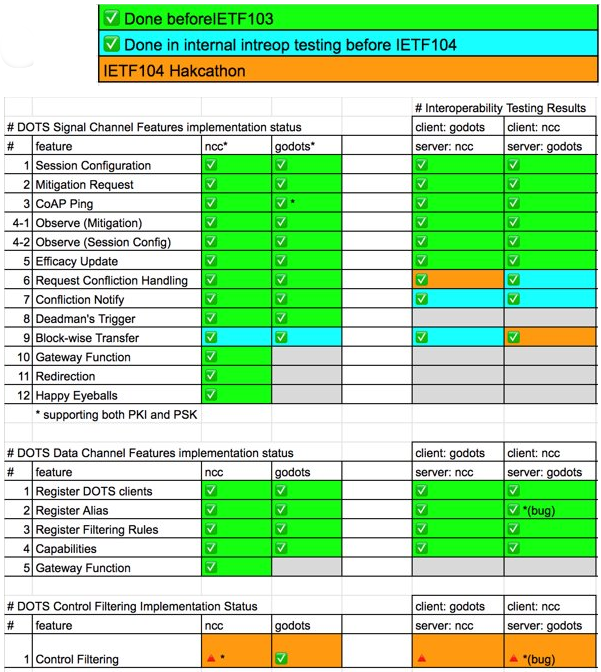
\includegraphics[scale=0.6]{Seminar-Template/Talk7/images/features_interoperability.png}}
\centering
\caption{Interoperable features tested during IETF104 Hackathon (2019)}
\end{figure}

\subsection{Challenges}

While implementing their solutions, NTT, NCC and Arbor Networks stated certain difficulties in either realizing the drafts or the viability of the drafts themselves. For example, while the DOTS drafts specify RESTCONF as the data channel protocol, go-dots and NCC DOTS use CoAP, because a suitable RESTCONF library does not exist \cite{hackathon-99}. Similarily Arbor Networks stated that even a suitable CoAP library proved difficult to find for their Python-based implementation \cite{arbor-101}.

One problem that was challenged recently, is the heartbeat mechanism of DOTS. Since the draft called for CoAP-based heartbeat mechanisms over unreliable transports (UDP) the planned retransmission related parameters would be void if a connection was made using a reliable transport (TCP) because CoAP over reliable transport does not support confirmable or non-confirmable message types \cite{heartbeat-challenge}. The solution to this problem was introduced at the next IETF Conference. By introducing DOTS-specific heartbeat messages in the protocol, the heartbeat drawbacks of CoAP were mitigated \cite{heartbeat-solution}.

During IETF 105, China Mobile presented their issues regarding deployment requirements of DOTS-powered infrastructures as an ISP \cite{china-mobile-105}. While the architecture draft specifies some scenarios how DOTS could be used, infrastructures are often much more complex. Their argument was that the drafts do not specify how exactly mitigation should be handled, especially in hierarchical networks where it is not clear which DOTS Clients calls for different DOTS Servers depending on type and load of attack \cite{chen-deployment}.

%%-----------------------------------------------------------------

\section{Discussion, Comparison \& Conclusion}

% Summarize and discuss the key points of the other chapters.

Since DOTS specifies only the necessary parties and the protocol that runs between them, comparing DOTS to existing DDoS mitigation solutions is difficult. Products offered by companies like Cloudflare and Akamai consist of a multitude of components, the communication protocol between a customer and a supplier only being a small fraction of it. One could argue that due to the freedom in configuring and setting up the infrastructure, DOTS enables much more user- and use-case specific installations of DDoS mitigation infrastructure. For example, should enough DDoS-mitigation hardware manufacturers choose to adapt DOTS, setting up infrastructures consisting of different products will be much easier.

At the beginning of this paper, we categorized existing solutions into four categories and characterized how they typically work. We shall visit these types of DDoS mitigation use cases and propose an assessment of DOTS with respect to these use cases. First we consider the on-premise centralized DDoS mitigation scenario. This scenario often involves simple mitigation techniques such as destination based filtering using a firewall. With this, frequent and simple attacks can be mitigated successfully. However, for attacks that exceed the capacities of such systems in scale or complexity usually involve the orchestration of multiple systems in a distributed manner. Once we recognize this distributed nature of defending the attack, there is a clear need for an effective, cooperative mitigation service communicating over signaling channels. Most research in this area focuses on the mitigation techniques, thus it makes sense to define a standardized approach for signaling between mitigation systems. Mitigation attacks in a distributed, but on-premise manner is targeted within DOTS by the DDoS Orchestration use case as described in section \ref{goals}. Conceptually, DOTS provides all components to support this scenario. It is our assessment that the complexity introduced by the architecture of DOTS will not be applicable to all distributed mitigation scenarios. The main benefit provided by DOTS is that the signaling was carefully designed to work under attack conditions and that it is an open standard. 

Consequentially, one could reason that since DOTS is an open standard, on-premise mitigation systems were suddenly compatible with off-premise distributed mitigation systems. As our literature review revealed, the commercial providers of such off-premise distributed mitigation systems have already gained high adoption and are continuing to gain attraction. As outlined in one of the use cases, the victim site could interact with a third-party DMS through the DOTS signaling channel. DOTS could provide all required features from authentication to mitigation to satisfy customers of this use case. Our literature review revealed that these providers employ different mitigation and traffic diversion techniques. This is where DOTS allows a lot of room to such commercial providers, making the standard an interesting opportunity to both the providers and customers of such DMS. In addition to the operation and adoption of such DMS providers, we have also learned about the customers of those services. This is important to note since many customers do not actually engage with their DMS provider in a dynamic manner. The DDoS protection can be characterized as an always-on solution which continuously protects infrastructure such as web sites. Such customers would likely not profit directly from the DOTS standard since one can even imagine that they are not knowledgeable about DDoS attacks.

An emerging scenario is the defense among decentralized actors. This opens up a number of advantages such as the pooling of capacities or mitigation techniques that are being applied closer to the source, such as egress filtering provided by a number of autonomous systems. There is ongoing research in this area and the adoption of commercial services is not described in literature (??). The recursive relationships as they are provided within DOTS allow that DOTS can be used in this context as well. Although a decentralized attack mitigation could be achieved, DOTS is not a peer-to-peer protocol. To achieve something like that, a fully meshed setup between all peers would have to be established or the recursive relationships would have to span the whole network. It is unclear whether this condition will introduce a complexity that makes a decentralized approach infeasible, or not. After all, there exist other protocols, such as for example eBGP, that are already used between autonomous systems to provide the global routing. With DOTS, one would have fine-grained control over the protection of services and relationships between actors.

To conclude, we can see that the DOTS standard is applicable to a number of scenarios that have been showcased to function with existing implementation that work in various configurations. Most prominently distributed and decentralized mitigation solutions and services are conceptually compatible. However, the complex nature of the DOTS architecture will only pay off for certain scenarios.

%%-----------------------------------------------------------------
\begin{thebibliography}{99}
\bibitem {leitfaden} Martin Waldburger, Patrick Poullie, Burkhard Stiller: \emph{Guideline for Seminar Reports}, Communication Systems Group, Department of Infromatics, University of Zurich, January 2013. \url{http://www.csg.uzh.ch/teaching/guideline-seminar-report-v05.pdf}.

\bibitem{DoS-Explained} What is a Denial-of-Service (DoS) Attack? Cloudflare, Accessed: 17. March 2020 \url{https://www.cloudflare.com/learning/ddos/glossary/denial-of-service/}

\bibitem{DoS-Norton} What are Denial of Service (DoS) attacks? DoS attacks explained, Steve Weisman for NortonLifeLock, Accessed: 17. March 2020 \url{https://us.norton.com/internetsecurity-emerging-threats-dos-attacks-explained.html}

\bibitem{DoS-PCWelt} Drei Angriffsarten, Alfredo Vistola, Accessed: 17. March 2020 \url{https://www.pcwelt.de/ratgeber/Drei-Angriffsarten-DoS-DDoS-Denial-of-Service-6187646.html}

\bibitem{DoS-PaloAlto} What is a denial of service attack (DoS) ?,  Accessed: 17. March 2020 \url{https://www.paloaltonetworks.com/cyberpedia/what-is-a-denial-of-service-attack-dos}

\bibitem{DoS-Comparitech} Dos vs DDoS Attacks: The Differences and How To Prevent Them, TIM KEARY,  Acessed: 24. March 2020 \url{https://www.comparitech.com/net-admin/dos-vs-ddos-attacks-differences-prevention/#What_is_a_DoS_Attack}

\bibitem{PingOfDeath-Cloudflare} Ping of Death DDoS attack, Accessed: 24. March 2020 \url{https://www.cloudflare.com/learning/ddos/ping-of-death-ddos-attack/}

\bibitem{DoS-Teardrop} DDoS Attack Definitions - DDoSPedia, Accessed: 22. March 2020 \url{https://security.radware.com/ddos-knowledge-center/ddospedia/teardrop-attack/}

\bibitem{nazario2008ddos} DDoS attack evolution, Nzario, Jose, Network Security, 2008, \url{https://doi.org/10.1016/S1353-4858(08)70086-2}

\bibitem{DDoS-MELANI} DDoS Attacken, Accessed: 24. March 2020 \url{https://www.melani.admin.ch/melani/de/home/themen/DDoSAttacken.html}

\bibitem{Botnet-ReadWrite} How To Build A Botnet In 15 Minutes, Brian Proffitt, Accessed: 24. March 2020 \url{https://readwrite.com/2013/07/31/how-to-build-a-botnet-in-15-minutes/}

\bibitem{IPSpoofing} What is IP spoofing?, Cloudflare, Accessed: 17. March 2020 \url{https://www.cloudflare.com/learning/ddos/glossary/ip-spoofing/}

\bibitem{Shadowserver} Open Simple Service Discovery Protocol (SSDP) Scanning Project, Accessed: 24. March 2020 \url{https://scan.shadowserver.org/ssdp/index.html}

\bibitem{CloudFlare-FamousDDoS} Famous DDoS Attacks | The Largest DDoS Attacks Of All Time, Accessed 24. March 2020 \url{https://www.cloudflare.com/learning/ddos/famous-ddos-attacks/}

\bibitem{CloudFlare-Memcached} Memcached DDoS Attack, Accessed: 24. March 2020 \url{https://www.cloudflare.com/learning/ddos/memcached-ddos-attack/}

\bibitem{Cloudflare-SSDP} SSDP DDoS Attack, Accessed: 26. March 2020 \url{https://www.cloudflare.com/learning/ddos/ssdp-ddos-attack/}

\bibitem{Cloudflare-NTP} NTP Amplification DDoS Attack, Accessed: 26. March 2020 \url{https://www.cloudflare.com/learning/ddos/ntp-amplification-ddos-attack/}

\bibitem{Imperva-NTP} NTP Amplification, Accessed: 26. March 2020 \url{https://www.imperva.com/learn/application-security/ntp-amplification/}

\bibitem{Cloudflare-ApplicationLayer}Application Layer DDoS Attack Accessed: 26. March 2020 \url{https://www.cloudflare.com/learning/ddos/application-layer-ddos-attack/}

\bibitem{Cloudflare-HTTP} HTTP Flood Attack, Accessed: 26. March 2020 \url{https://www.cloudflare.com/learning/ddos/http-flood-ddos-attack/}

\bibitem{Cloudflare-DNSFlood} What is a DNS Flood? | DNS Flood DDoS Attack, Accessed: 26. March 2020 \url{https://www.cloudflare.com/learning/ddos/dns-flood-ddos-attack/}

\bibitem{Cloudflare-DNSAmplification} DNS Amplification Attack Accessed: 26. March 2020 \url{https://www.cloudflare.com/learning/ddos/dns-amplification-ddos-attack/}

\bibitem{ReflectionVSAmplification} Reflection Attacks and Amplification Attacks, Accessed: 26 March 2020 \url{https://www.cloudbric.com/blog/2015/03/reflection-attacks-and-amplification-atttacks/}

\bibitem{Cloudflare-UDP} UDP Flood Attack, Accessed: 26. March 2020 \url{https://www.cloudflare.com/learning/ddos/udp-flood-ddos-attack/}

\bibitem{Hostingtribunal-DDoSStatistics} 39 Jaw-Dropping DDoS Statistics to Keep in Mind for 2020, Accessed: 26. March 2020 \url{https://hostingtribunal.com/blog/ddos-statistics}

\bibitem{Metacompliance-DDoSStatistics} 310 Biggest DDoS Attacks and how your organisation can learn from them, Accessed: 26. March 2020 \url{https://www.metacompliance.com/blog/10-biggest-ddos-attacks-and-how-your-organisation-can-learn-from-them/}

\bibitem{Arstechnica-DDoSStatistics} US service provider survives the biggest recorded DDoS in history, Accessed: 26. March 2020 \url{https://arstechnica.com/information-technology/2018/03/us-service-provider-survives-the-biggest-recorded-ddos-in-history/}

\bibitem{Statista-MobileInternetSpeed}Durchschnittliche Download-Geschwindigkeit im Schweizer Mobilfunknetz 2019, Accessed: 26. March 2020 \url{https://de.statista.com/statistik/daten/studie/416684/umfrage/durchschnittliche-internetgeschwindigkeit-in-dach/}

\bibitem{Computerbase-Datarate}Durchschnittliche Weltrekord: Deutscher Internet-Knoten DE-CIX erreicht 9,1 Terabit/s, Sven Bauduin, 11.3.2020, Accessed: 26. March 2020 \url{https://www.computerbase.de/2020-03/de-cix-internet-knoten-9-terabits-traffic-weltrekord/}

\bibitem{Cisco-DDoSStatistics}Cisco Annual Internet Report (2018–2023) White Paper, Updated 9.3.2020, Accessed: 26. March 2020 \url{https://www.cisco.com/c/en/us/solutions/collateral/executive-perspectives/annual-internet-report/white-paper-c11-741490.html/}

\bibitem{ZDNet-DDoSStatistics}16 DDoS attacks take place every 60 seconds, rates reach 622 Gbps, Charlie Osborne, 18.02.2020, Accessed: 26. March 2020 \url{https://www.zdnet.com/article/16-ddos-attacks-take-place-every-60-seconds-rates-reach-622-gbps/}

\bibitem{Helpnetsecurity-DDoSStatistics}Across-the-board increase in DDoS attacks of all sizes, Accessed: 27. March 2020 \url{https://www.helpnetsecurity.com/2020/03/27/ddos-attacks-increase-2020/}

\bibitem{Securelist-DDoSStatistics}DDoS attacks in Q4 2018, Oleg Kupreev, Ekaterina Badovskaya, Alexander Gutnikov, 07.02.2019, Accessed: 27. March 2020 \url{https://securelist.com/ddos-attacks-in-q4-2018/89565/}

\bibitem{Corero-MultivectorDDoS}Understanding and Stopping Multi-Vector DDoS Attacks, Sean Newman, Accessed: 27. March 2020 \url{https://www.corero.com/blog/understanding-and-stopping-multi-vector-ddos-attacks/}

\bibitem{Symantec-MultivectorDDoS}Multi-Vector DOS Attacks Turning into the New Normal, Robert Lemos, 09.02.2018, Accessed: 27. march 2020 \url{https://symantec-blogs.broadcom.com/blogs/expert-perspectives/multi-vector-dos-attacks-turning-new-normal}

\bibitem{Techradar-DDoSStatistics}DDoS attacks could cost the UK \£1bn this year, Mike Moore, 21.03.2019, Accessed: 29. March 2020 \url{https://www.techradar.com/news/ddos-attacks-could-cost-the-uk-pound1bn-this-year}

\bibitem{Securelist-DDoSCosts}Was kostet eine DDoS-Attacke, Denis Markushin, 23.03.2017, Accessed: 29. March 2020 \url{https://de.securelist.com/the-cost-of-launching-a-ddos-attack/72496/}

\bibitem{Forbes-DDoSCosts}FBI Crackdown Leads To Massive Drop In DDoS Attacks, Lee Mathews, 19.03.2019, Accessed: 29. March 2020 \url{https://www.forbes.com/sites/leemathews/2019/03/19/fbi-crackdown-leads-to-massive-drop-in-ddos-attacks/#1a08d67ca49c}

\bibitem{dots-use-cases} Use cases for DDoS Open Threat Signaling, last accessed 30.03.2020, \url{https://tools.ietf.org/html/draft-ietf-dots-use-cases-20}

\bibitem{dots-architecture} Distributed Denial-of-Service Open Threat Signaling (DOTS) Architecture, last accessed 24.03.2020, \url{https://datatracker.ietf.org/doc/draft-ietf-dots-architecture/18}

\bibitem{dots-signal-channel} Distributed Denial-of-Service Open Threat Signaling (DOTS) Signal Channel Specification, last accessed 24.03.2020,
\url{https://datatracker.ietf.org/doc/draft-ietf-dots-signal-channel/41}

\bibitem{Cloudflare-DDoSMitigation}What is DDoS Mitigation?, Accessed: 31. March 2020 \url{https://www.cloudflare.com/learning/ddos/ddos-mitigation/}

\bibitem{Wired-DDoSMitigation}The 5 Essentials of DDoS Mitigation, Marc Gaffan, Accessed: 31. March 2020 \url{https://www.wired.com/insights/2012/12/the-5-essentials-of-ddos-mitigation/}

\bibitem{DDoS-MitigationSurvey}A survey of defense mechanisms against distributed denial of service (DDoS) flooding attacks, Zargar, Saman Taghavi and Joshi, James and Tipper, David, 2013, Accessed: 31. March 2020 \url{DOI: 10.1109/SURV.2013.031413.00127}

\bibitem{DetectionTechniques}Detection techniques of DDoS attacks: A survey, P. Kamboj, M. C. Trivedi, V. K. Yadav and V. K. Singh, 2017 4th IEEE Uttar Pradesh Section International Conference on Electrical, Computer and Electronics (UPCON), \url{DOI: 10.1109/UPCON.2017.8251130}

\bibitem{bgprouting} IETF: A Border Gateway Protocol 4 (BGP-4), \url{https://tools.ietf.org/html/rfc4271}, last accessed 31.03.2020

\bibitem{dps-adoption} Measuring the Adoption of DDoS Protection Services: Mattijs Jonker, Anna Sperotto, Roland van Rijswijk-Deij, Ramin Sadre, and Aiko Pras. 2016. In Proceedings of the 2016 Internet Measurement Conference (IMC ’16). Association for Computing Machinery, New York

\bibitem{blockchain-collaborative-defense} Cooperative Signaling of DDoS Attacks in a Blockchain-based Network: Bruno Rodrigues and Burkhard Stiller. 2019. 


\bibitem{DDoS-Radware}How to Recover from a DDoS Attack, Eyal Arazi, 19.11.2019, Accessed: 5. April 2020 \url{https://blog.radware.com/security/ddos/2019/11/how-to-recover-from-a-ddos-attack/}

\bibitem{ciscodecentralizedddos} Effective DDoS Mitigation in Distributed Peering Environments, \url{https://www.cisco.com/c/en/us/solutions/service-provider/network-infrastructure/ddos-mitigation-in-distributed-peering-environments.html#~white-paper}, last accessed 15.03.2020

\bibitem{go-dots-github} go-dots GitHub Repository, \url{https://github.com/nttdots/go-dots}, last accessed 23.4.2020

\bibitem{interop-100} DOTS Interoperability Report during IETF 100 Hackathon (2017), \url{https://datatracker.ietf.org/meeting/100/materials/slides-100-dots-hackathon-and-interoperability-test-report-00}, last accessed 23.4.2020

\bibitem{telemetry-draft} DOTS Telemetry Draft, \url{https://datatracker.ietf.org/doc/draft-ietf-dots-telemetry/}, last accessed 23.4.2020

\bibitem{hackathon-106} Telemetry-Related Hackathon activity report, \url{https://datatracker.ietf.org/meeting/106/materials/slides-106-dots-dots-telemetry-related-hackathon-activity-report-00.pdf}, last accessed 23.4.2020

\bibitem{hackathon-99} DOTS 99 Hackathon Go Implementation, \url{https://datatracker.ietf.org/meeting/99/materials/slides-99-dots-dots-hackathon-report-00.pdf}, last accessed 23.4.2020

\bibitem{ncc-public-server} NCC DOTS public server description, \url{https://trac.ietf.org/trac/dots/wiki}, last accessed 23.4.2020

\bibitem{interop-101} DOTS Interoperability Report during IETF 101 Hackathon (2017), \url{https://datatracker.ietf.org/meeting/101/materials/slides-101-dots-ietf-101-hackathon-dots-interop-01}, last accessed 23.4.2020

\bibitem{interop-103} DOTS I,teroperability Report during IETF 103 Hackathon (2018), \url{https://datatracker.ietf.org/meeting/103/materials/slides-103-dots-interop-report-from-ietf-103-hackathon-00.pdf}, last accessed 23.4.2020

\bibitem{ncc-implementation} NCC DOTS Implementation Presentation, \url{https://datatracker.ietf.org/meeting/101/materials/slides-101-dots-ncc-group-implementation-report-00.pdf}, last accessed 23.4.2020

\bibitem{arbor-101} Arbor Networks' DOTS Presentation during IETF 101 Hackathon (2017), \url{https://datatracker.ietf.org/meeting/101/materials/slides-101-dots-arbor-networks-implementation-report-00.pdf}, last accessed 23.4.2020

\bibitem{interop-102} DOTS Interoperability Report during IETF 102 Hackathon (2018), \url{https://datatracker.ietf.org/meeting/102/materials/slides-102-dots-ietf-102-hackathon-interop-report-00.pdf}, last accessed 23.4.2020

\bibitem{interop-104} DOTS Interoperability Report during IETF 104 Hackathon (2019), \url{https://datatracker.ietf.org/meeting/104/materials/slides-104-dots-interoperability-and-hackathon-report-00.pdf}, last accessed 23.4.2020

\bibitem{bcp14} S. Bradner: Key words for use in RFCs to Indicate Requirement Levels \url{https://www.rfc-editor.org/bcp/bcp14}, last accessed 23.4.2020

\bibitem{rfc8612} A. Mortensen, Arbor Networks, T. Reddy, McAfee, R. Moskowitz, Huawei: DDoS Open Threat Signaling (DOTS) Requirements, \url{https://www.rfc-editor.org/rfc/rfc8612.html}, last accessed 23.4.2020

\bibitem{rfc791} RFC 791 - Internet Protocol \url{https://tools.ietf.org/html/rfc791#page-25}, last accessed 23.4.2020

\bibitem{heartbeat-challenge} IETF 105 DOTS Heartbeat Mechanism, \url{https://datatracker.ietf.org/meeting/105/materials/slides-105-dots-heartbeat-mechanism-mirjas-discuss-on-the-signal-channel-i-d-00.pdf}, last accessed 23.4.2020

\bibitem{heartbeat-solution} IETF 106 DOTS Heartbeat Mechanism Update, \url{https://datatracker.ietf.org/meeting/106/materials/slides-106-dots-dots-signal-channel-heartbeat-mechanism-update-00.pdf}, last accessed 23.4.2020

\bibitem{china-mobile-105} IETF 105 DOTS Server Deployment Considerations, \url{https://datatracker.ietf.org/meeting/105/materials/slides-105-dots-dots-server-deployment-consideration-00.pdf}, last accessed 23.4.2020

\bibitem{chen-deployment} DOTS Server Hierarchichal Deployment, \url{https://tools.ietf.org/pdf/draft-chen-dots-server-hierarchical-deployment-02.pdf}, last accessed 23.4.2020

\end{thebibliography}